\documentclass[10pt,aspectratio=169]{beamer}

\usetheme[progressbar=frametitle]{metropolis}
\usepackage{appendixnumberbeamer}
\usepackage[absolute,overlay]{textpos}
\usepackage{booktabs}
\usepackage[scale=2]{ccicons}
\usepackage{tikz}
\usepackage{pgfplots}
\usepackage{listings}
\usepgfplotslibrary{dateplot}

\usepackage{xspace}
\newcommand{\themename}{\textbf{\textsc{metropolis}}\xspace}
\usecolortheme{default}
% Colores defined
\usepackage{color}
\definecolor{White}{HTML}{ffffff}
\definecolor{Blue}{HTML}{183354}
\definecolor{Gray}{HTML}{e6e6e6} % d6d6d6
\definecolor{Orange}{HTML}{ff8000}
\definecolor{OrangeBackground}{HTML}{fff3e6}

\definecolor{dkgreen}{rgb}{0,0.6,0}
\definecolor{gray}{rgb}{0.5,0.5,0.5}
\definecolor{mauve}{rgb}{0.58,0,0.82}
\definecolor{darkgray}{RGB}{96, 98, 99}
\definecolor{darkred}{RGB}{145, 29, 16}


% Some boxes
\setbeamercolor{coloredboxstuff}{fg=black,bg=Gray}
\setbeamercolor{boxorange}{fg=black,bg=Orange}

% Change colores template
\setbeamercolor{background canvas}{bg=White}
\setbeamercolor{title}{fg=Blue}
\setbeamercolor{frametitle}{bg=Blue}
\setbeamercolor{item}{fg=orange}
\setbeamercolor{normal text}{fg=black}
\usebeamercolor[fg]{normal text}

\newcommand<>{\reveal}[1]{\mbox{}\visible#2{#1}}

\newcommand\Fontvi{\fontsize{10}{7.2}\selectfont}
\newcommand\Fonteight{\fontsize{9pt}{7.2}\selectfont}


\usepackage{lmodern,amsmath,amssymb}
\usepackage[beamer]{hf-tikz}
\usepackage{xcolor}
\usepackage{soul}
\newcommand{\hll}[1]{\colorbox{orange!10}{$\displaystyle #1$}}

\addtobeamertemplate{title}{\vskip-10.5ex}{}

\usepackage{listings}
\lstset{
	language=R,
	aboveskip=3mm,
	belowskip=3mm,
	showstringspaces=false,
	belowskip=0.15cm,
	% belowcaptionskip=0\baselineskip,
	columns=fullflexible,
	basicstyle={\fontsize{8}{9.6}\ttfamily},
	frame=single,
	xleftmargin=3mm,
	xrightmargin=1mm,
	% framerule=1pt,
	rulecolor=\color{black},
	numbers=left,
	stepnumber=1,
	numbersep=5pt,
	tabsize=2,
	numberstyle=\tiny\color{darkred},
	keywordstyle=\color{mauve},
	commentstyle=\color{darkgray},
	stringstyle=\color{dkgreen},
	breaklines=true,
	breakatwhitespace=false,
	captionpos=b,
	deletekeywords={
		model, 
		data, 
		example,
		single, 
		real, 
		min, 
		frame, 
		file, 
		by, 
		log, 
		density, 
		labels,
		cov,
		\_,
		se
	},
	morekeywords={
		deconvDigitalDLSorter, 
		deconvDigitalDLSorterObj, 
		loadRealSCProfiles, 
		loadFinalSCProfiles, 
		estimateZinbwaveParams, 
		simSingleCellProfiles, 
		generateTrainAndTestBulkProbMatrix, 
		install\_, 
		github,
		showProbPlot,
		generateBulkSamples,
		loadDeconvData,
		prepareDataForTraining,
		trainDigitalDLSorterModel,
		calculateEvalMetrics,
		barPlotCellTypes,
		distErrorPlot,
		corrExpPredPlot,
		blandAltmanLehPlot,
		barErrorPlot,
		loadDeconvDataFromSummarizedExperiment
	}
}

\usepackage{tikz}
\newsavebox\blockbox
\newenvironment{highlightblock}{%
  \begin{lrbox}{\blockbox}%
    \begin{minipage}{.9\textwidth}
}{
    \end{minipage}
  \end{lrbox}
  \tikz\node[
    fill=OrangeBackground,
    draw=Orange,
    line width=1pt,
    inner sep=7.5pt,
    % rounded corners,
    outer sep=0pt,
    text centered
  ]{\usebox\blockbox};
}


\usepackage{hyperref}
\hypersetup{
    colorlinks=true,
    linkcolor=black,
    filecolor=magenta,
    citecolor=black, 
    urlcolor=magenta
}

%%%%%%%%%%%%%%%%%%%%%%%%%%%%%%%%%%%%%%%%%%%%%%%%%%%%%%%%%%%%%%%%%%%%%%%%%%%%%%%%%%%%
%%%%%%%%%%%%%%%%%%%%%%%%%%%%%%%%%%%%%% TITLE %%%%%%%%%%%%%%%%%%%%%%%%%%%%%%%%%%%%%%%
%%%%%%%%%%%%%%%%%%%%%%%%%%%%%%%%%%%%%%%%%%%%%%%%%%%%%%%%%%%%%%%%%%%%%%%%%%%%%%%%%%%%

\title{\textit{digitalDLSorteR}: paquete de R para la deconvolución de muestras \textit{bulk RNA-seq} basado en Redes Neuronales.}
\subtitle{Trabajo Fin de Máster\\Máster en Bioinformática y Biología Computacional}
% \date{\today}
\date{}
\author{Diego Mañanes Cayero}
\institute{Universidad Autónoma de Madrid \\
Curso 2019-2020}

\titlegraphic{%
\begin{picture}(0,0)
  \put(340,-170){\makebox(0,0)[rt]{
\includegraphics[height=1.6cm]{images/eps_logo.png}}}
  \put(145,-160){\makebox(0,0)[rt]{
\includegraphics[height=2cm]{images/logo_uam_mod_hor.png}}} % uam_logo_nuevo2.png
\end{picture}}

%%%%%%%%%%%%%%%%%%%%%%%%%%%%%%%%%%%%%%%%%%%%%%%%%%%%%%%%%%%%%%%%%%%%%%%%%%%%%%%%%%%%
%%%%%%%%%%%%%%%%%%%%%%%%%%%%%%%%%%%% COMIENZO %%%%%%%%%%%%%%%%%%%%%%%%%%%%%%%%%%%%%%
%%%%%%%%%%%%%%%%%%%%%%%%%%%%%%%%%%%%%%%%%%%%%%%%%%%%%%%%%%%%%%%%%%%%%%%%%%%%%%%%%%%%

\begin{document}

\maketitle

\begin{frame}{Contenidos}
  \setbeamertemplate{section in toc}[sections numbered]
  \tableofcontents%[hideallsubsections]
\end{frame}

%%%%%%%%%%%%%%%%%%%%%%%%%%%%%%%%%%%%%%%%%%%%%%%%%%%%%%%%%%%%%%%%%%%%%%%%%%%%%%%%%%%%
%%%%%%%%%%%%%%%%%%%%%%%%%%%%%%%%%% INTRODUCCIÓN %%%%%%%%%%%%%%%%%%%%%%%%%%%%%%%%%%%%
%%%%%%%%%%%%%%%%%%%%%%%%%%%%%%%%%%%%%%%%%%%%%%%%%%%%%%%%%%%%%%%%%%%%%%%%%%%%%%%%%%%%

\section[Introducción y contexto]{Introducción y contexto}

% Cáncer y micro-entorno tumoral ---------------------------------------------------

\subsection{1.1. Cáncer y heterogeneidad celular}

% \begin{frame}[fragile]{Cáncer y micro-entorno tumoral}
% \end{frame}

\begin{frame}[fragile]{Cáncer y micro-entorno tumoral}
  \begin{columns}
    \begin{column}{0.36\textwidth}
      \begin{textblock*}{1cm}(0.5cm,1.3cm)
        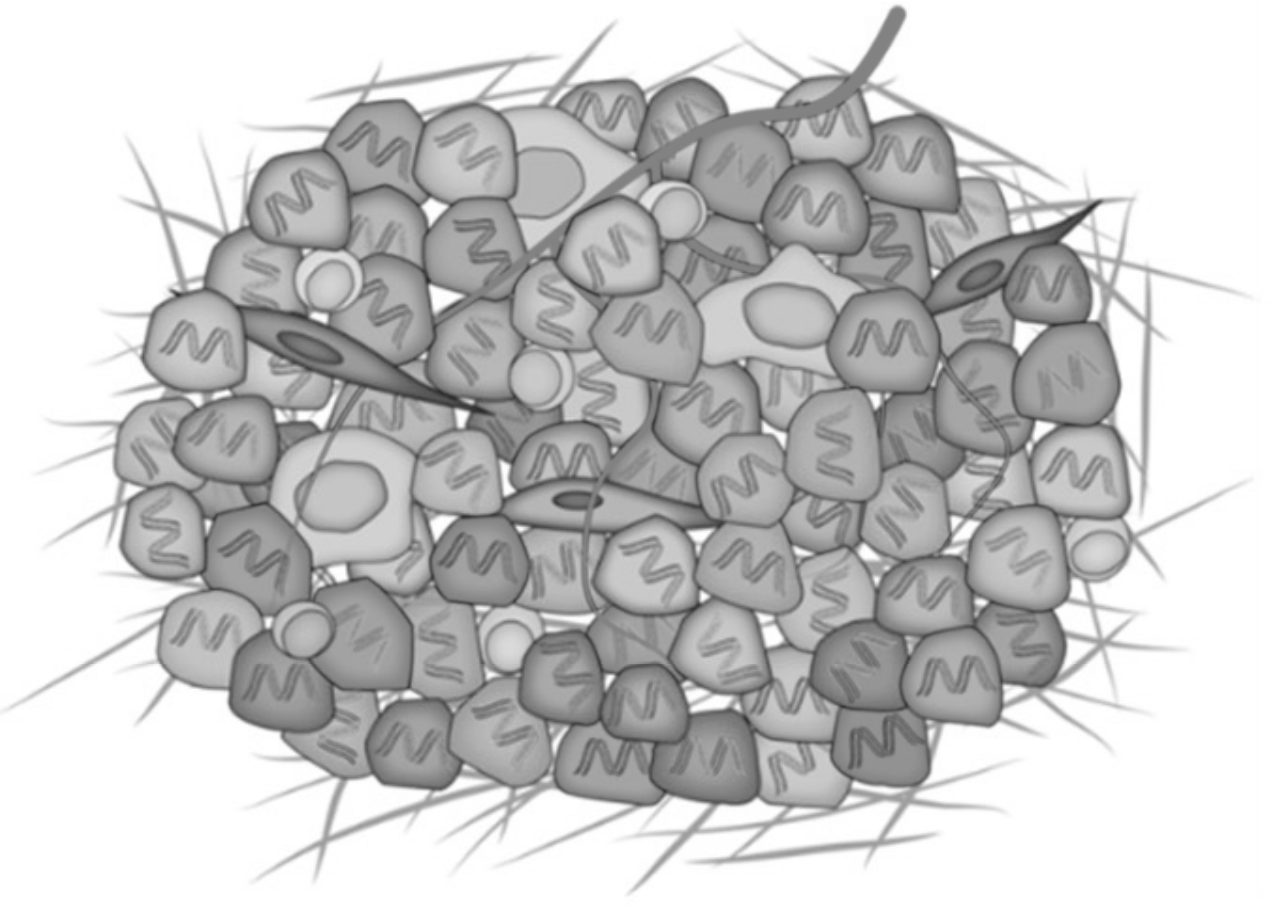
\includegraphics[scale=.8]{images/tumor_heterogenity_bw.png}
      \end{textblock*}
      \begin{textblock*}{5cm}(2.2cm,4.3cm)
        \includegraphics<2,3>[scale=0.05,width=1cm]{images/down_arrow.jpg}
      \end{textblock*}
      \begin{textblock*}{1cm}(0.5cm,5.3cm)
        \includegraphics<2,3>[scale=.8]{images/tumor_heterogenity_color.png}
      \end{textblock*}
    \end{column}

    \begin{column}{0.7\textwidth}
      \begin{overlayarea}{\linewidth}{1\textheight}
        \metroset{block=fill}
        \begin{block}{Por qué}
          \vskip0.5em
          \begin{itemize}
            \item Diferentes poblaciones tumorales.
            \item Micro-entorno tumoral: diferentes tipos \\ celulares con complejas interacciones.
            \item Sello de Identidad del cáncer.
          \end{itemize}
        \end{block}
        \metroset{block=fill}

        \only<2>{\begin{figure}
            \makebox(230,15)[rt]{\includegraphics<2>[height=4cm]{images/tumor_hallmarks_degradado_3.png}}
          \end{figure}}

        \only<3>{\begin{figure}
            \makebox(230,15)[rt]{\includegraphics<3>[height=4cm]{images/tumor_hallmarks_degradado_2.png}}
          \end{figure}}

      \end{overlayarea}
    \end{column}
  \end{columns}
\end{frame}


\begin{frame}[fragile]{Papel del sistema inmune en la enfermedad}
  \Fonteight
  \begin{alertblock}{Papel clave}
    \begin{itemize}
      \item La similitud entre células será máxima cuando sus $k$-vecinos son los
            mismos $\rightarrow$ mismo fenotipo.
      \item Similitud decaerá entre células que compartan menos vecinos conectados
            $\rightarrow$ distinto fenotipo.
    \end{itemize}
  \end{alertblock}

  \begin{alertblock}{Terapias}
    \begin{itemize}
      \item La similitud entre células será máxima cuando sus $k$-vecinos son los
            mismos $\rightarrow$ mismo fenotipo.
      \item Similitud decaerá entre células que compartan menos vecinos conectados
            $\rightarrow$ distinto fenotipo.
    \end{itemize}
  \end{alertblock}

  \begin{figure}
    \centering
    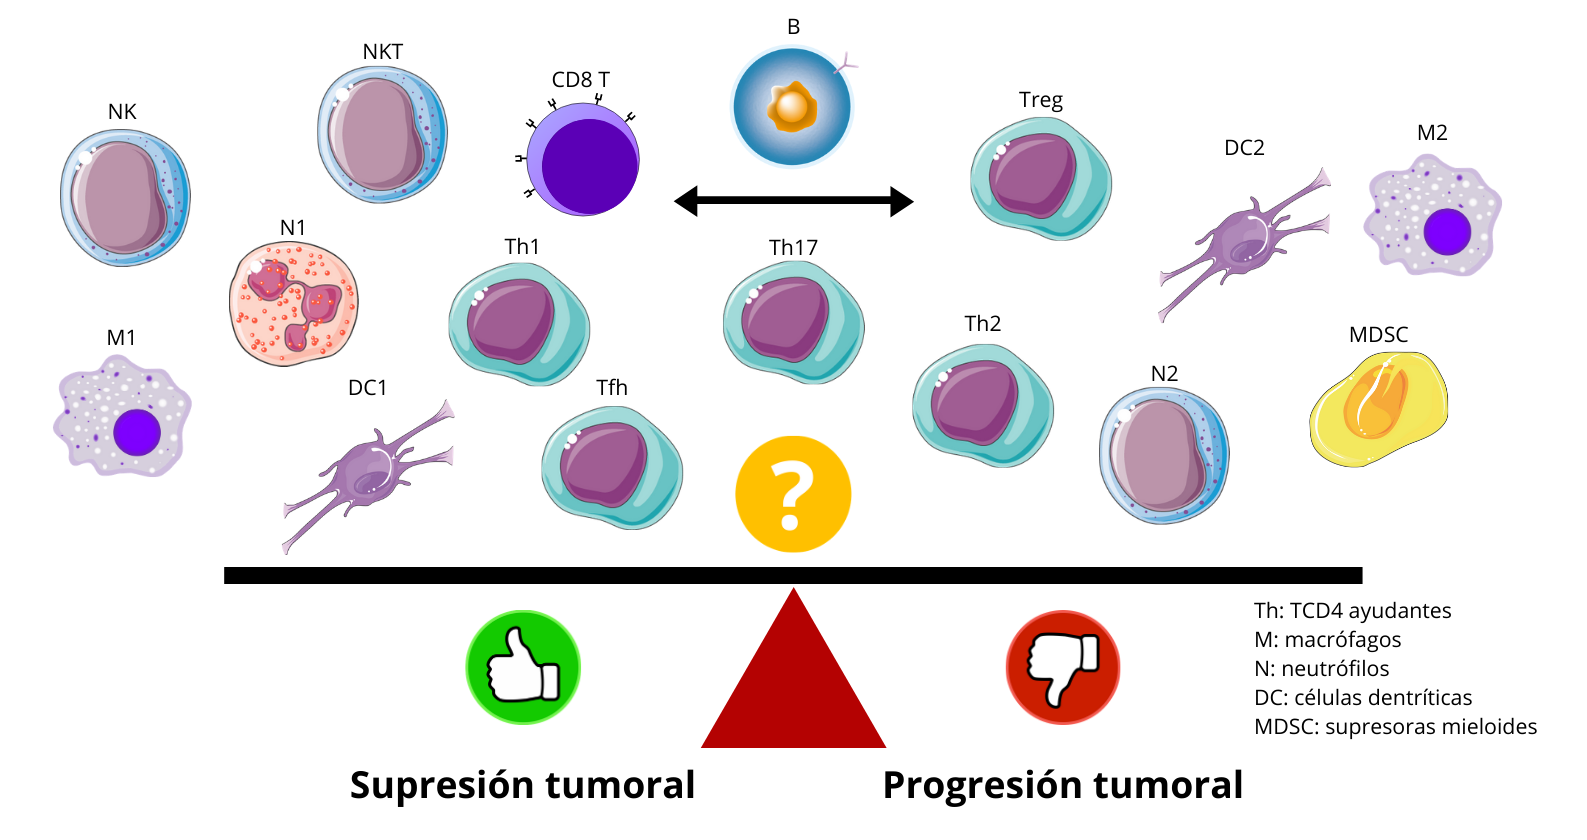
\includegraphics[width=7cm]{images/balance_Imm_2.png}
  \end{figure}

\end{frame}


\begin{frame}[fragile]{Caso de estudio: cáncer de mama}
  \vskip1em
  Enfermedad altamente \alert{\textbf{heterogénea desde el punto de vista molecular}}.
  \Fontvi
  \vskip0.5em
  \begin{columns}
    \begin{column}{0.5\textwidth}
      \vskip-0.5em
      \begin{alertblock}{Subtipos intrínsecos del cáncer}
        \vskip-0.5em
        \Fonteight{
          \begin{itemize}
            \item Luminal A (ER+).
            \item Luminal B (ER+/HER2+).
            \item HER2 enriquecido (HER2+).
            \item Triple negativo (TNBC).
          \end{itemize}
        }
      \end{alertblock}
      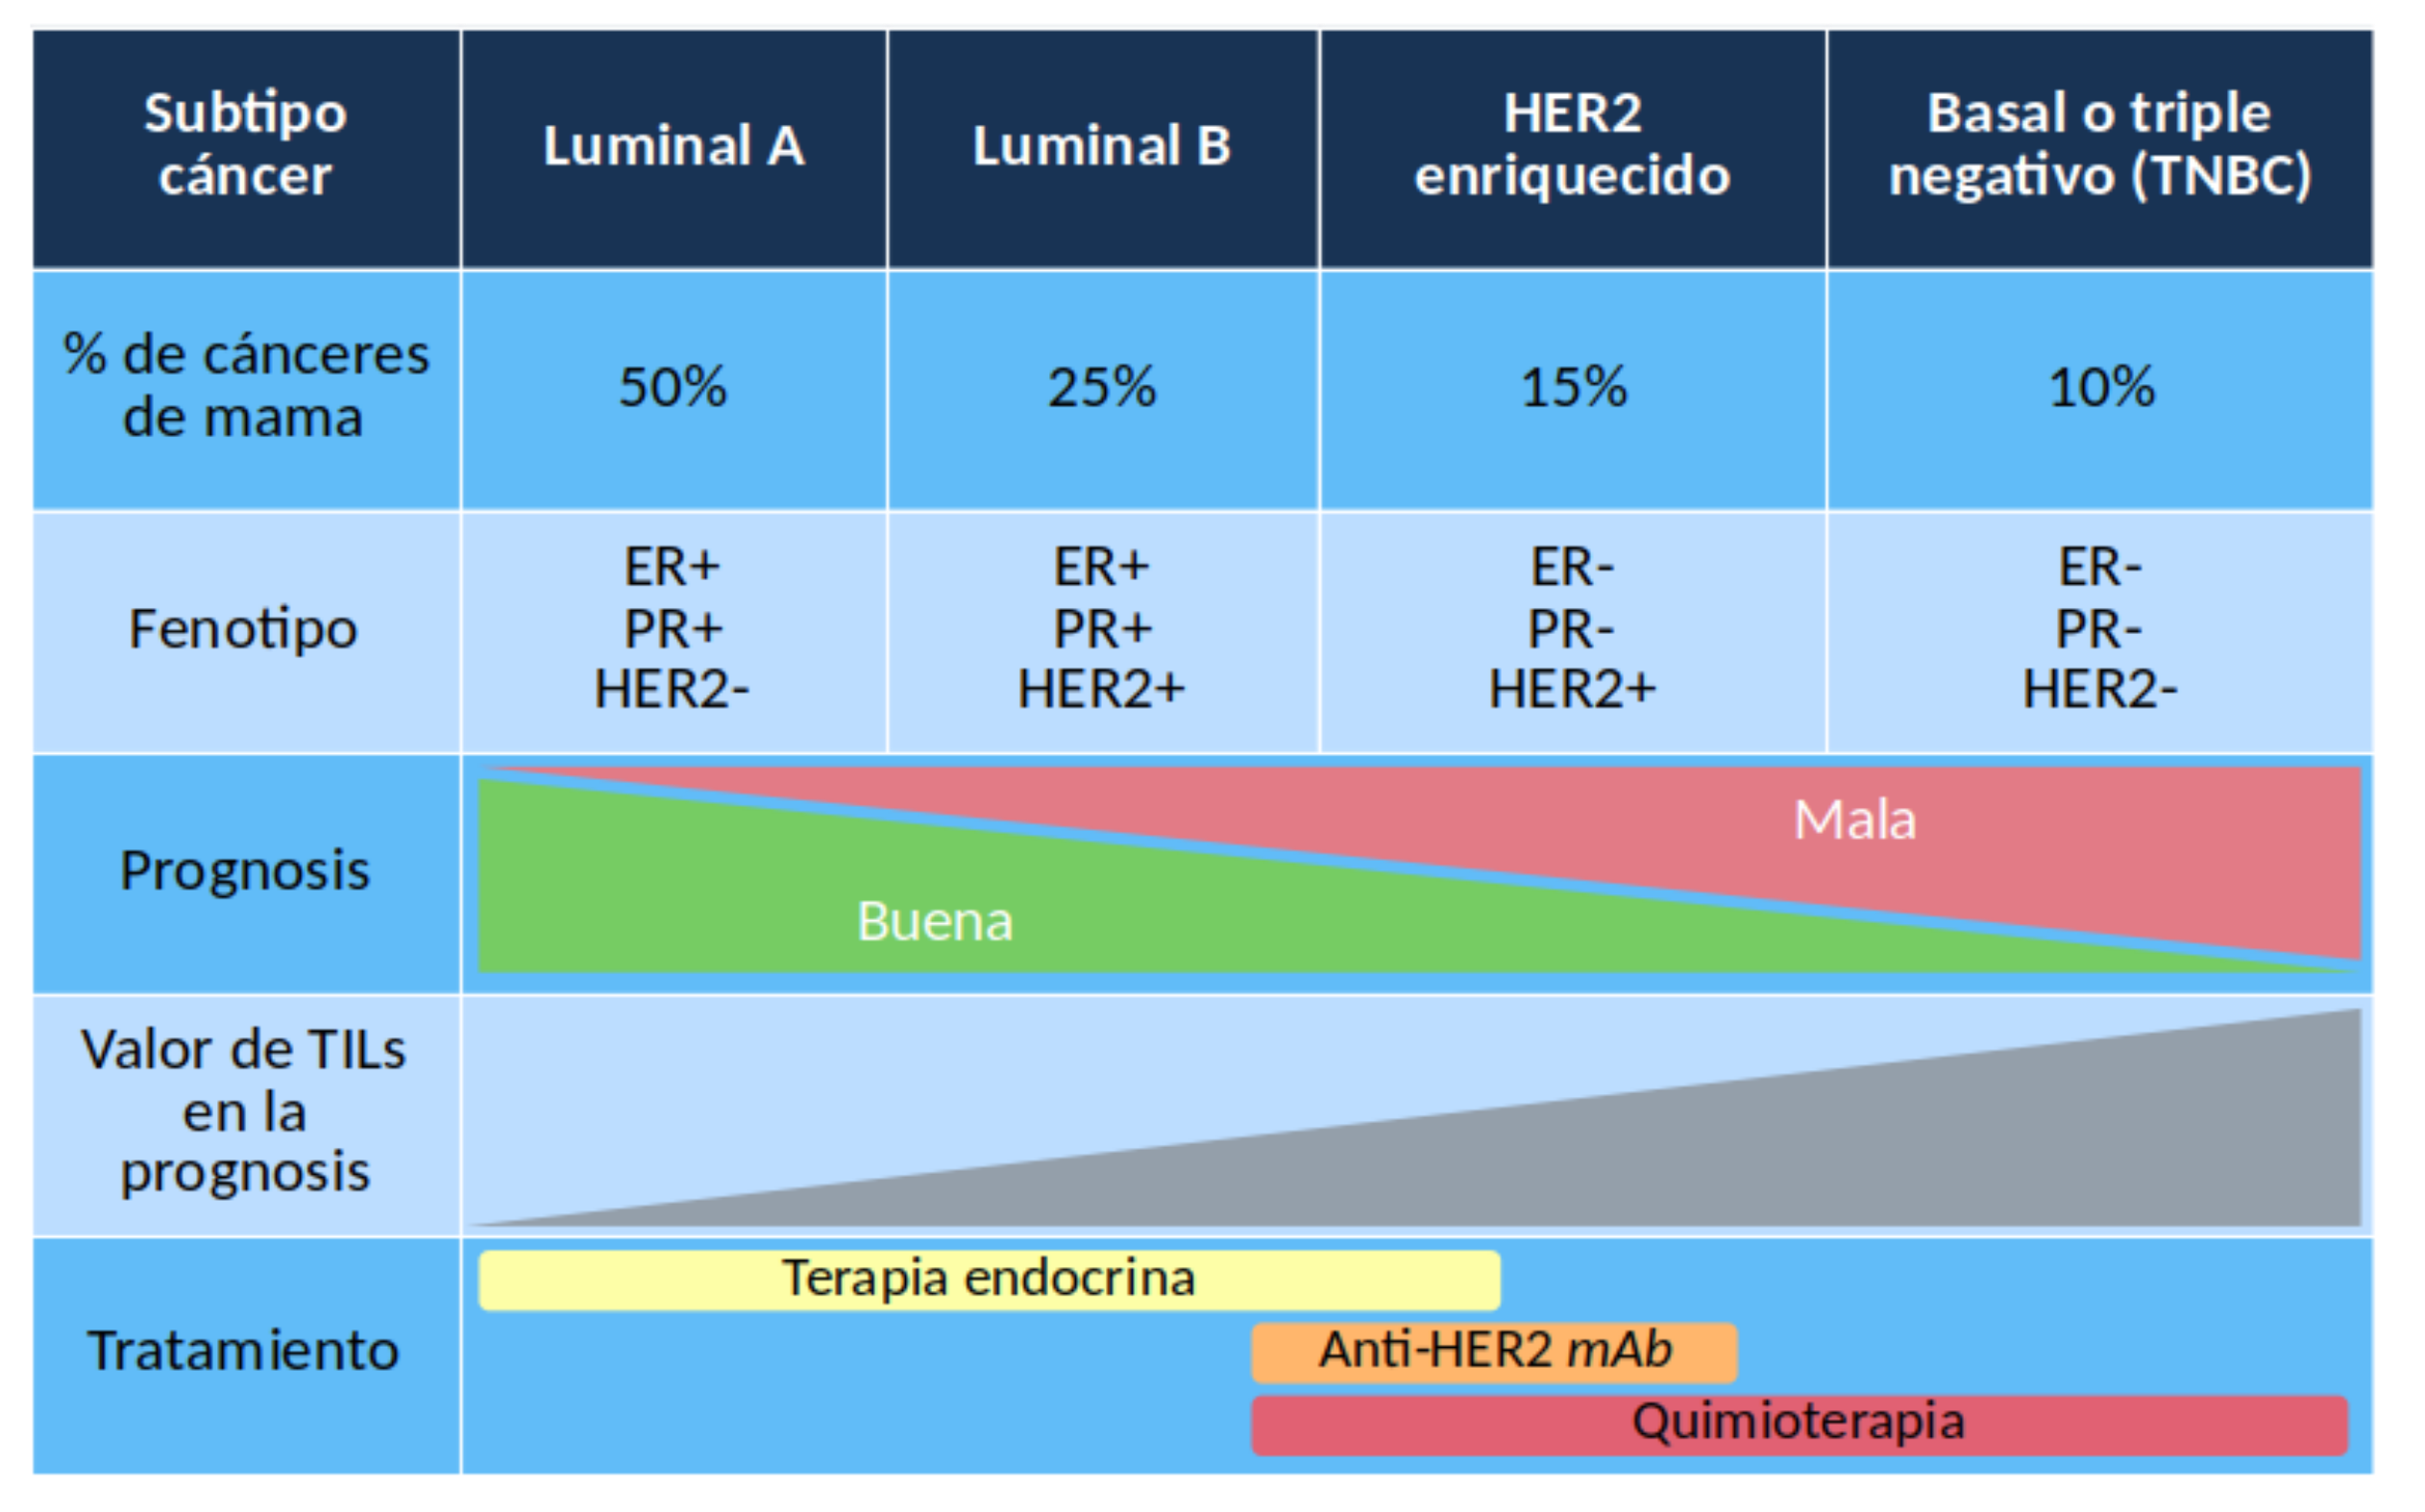
\includegraphics[width=7cm]{images/tabla_breast_2_mod.png}
    \end{column}
    \begin{column}{0.6\textwidth}
      \begin{alertblock}{Importancia de las células inmunes infiltradas}
        \vskip-0.5em
        \Fonteight{
          \begin{itemize}
            \item Luminal A (ER+).
            \item Luminal B (ER+/HER2+).
            \item HER2 enriquecido (HER2+).
            \item Triple negativo (TNBC).
          \end{itemize}
        }
      \end{alertblock}
    \end{column}
  \end{columns}
\end{frame}

% Tecnologías para estudiar células: scRNAseq --------------------------------------

\subsection{1.2. Tecnologías para explorar la heterogeneidad celular: \textit{scRNA-seq}}

\begin{frame}[fragile,t]{Estudio de la heterogeneidad celular}
  % \vskip0.5em
  Necesidad de métodos para el estudio de la heterogeneidad celular.
  % \Fontvi
  \vskip-0.7em
  % \begin{overlayarea}{\linewidth}{1\textheight}
  \begin{columns}
    \begin{column}{0.65\textwidth}
      \vskip-0.5em
      \begin{alertblock}{Tradicionalmente}
        \vskip1mm
        A nivel de proteína mediante técnicas inmunohistoquímicas, inmunofluorescencencia y citometría de flujo.
      \end{alertblock}
      \begin{alertblock}{Tecnologías de alto rendimiento}
        \vskip1mm
        A nivel transcriptómico mediante NGS: \textit{RNA-seq}.\\
        \vskip1mm
        Dos variantes:
      \end{alertblock}
    \end{column}

    \begin{column}{0.3\textwidth}
      \vskip7mm
      \begin{highlightblock}
        \centering
        \Fontvi{Pequeña combinación de marcadores génicos}
      \end{highlightblock}
      \vskip1mm
      \begin{highlightblock}
        \centering
        \Fontvi{Estatus funcional completo}
      \end{highlightblock}
    \end{column}

  \end{columns}

  \vskip-1.5em

  % Parte inferior
  \begin{columns}
    \begin{column}{0.7\textwidth}
      \Fontvi
      \begin{itemize}
        \item \textit{Bulk RNA-seq} (nivel tisular): los niveles de expresión corresponden al sumatorio de tipos celulares presentes en las muestras.
              \vskip5mm
        \item \textit{Single-cell RNA-seq} (nivel celular): los niveles de expresión corresponden a cada célula individual que compone la muestra.
      \end{itemize}
    \end{column}

    \begin{column}{0.3\textwidth}
      \begin{figure}
        \centering
        \hskip-4mm
        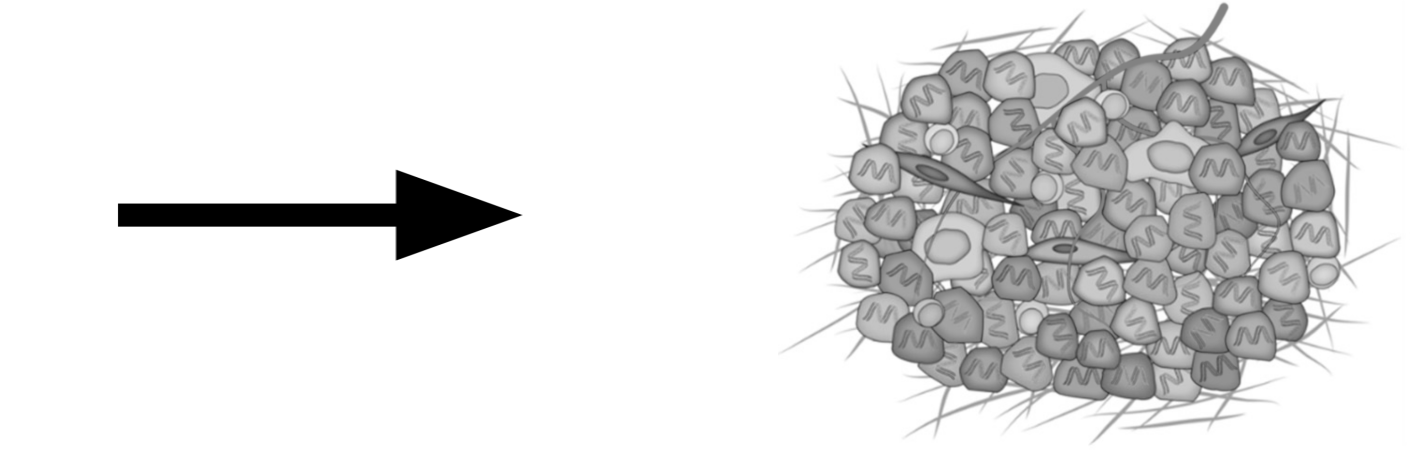
\includegraphics[width=4cm]{images/tumor_bw_arrow.png}\\
        \hskip-4mm
        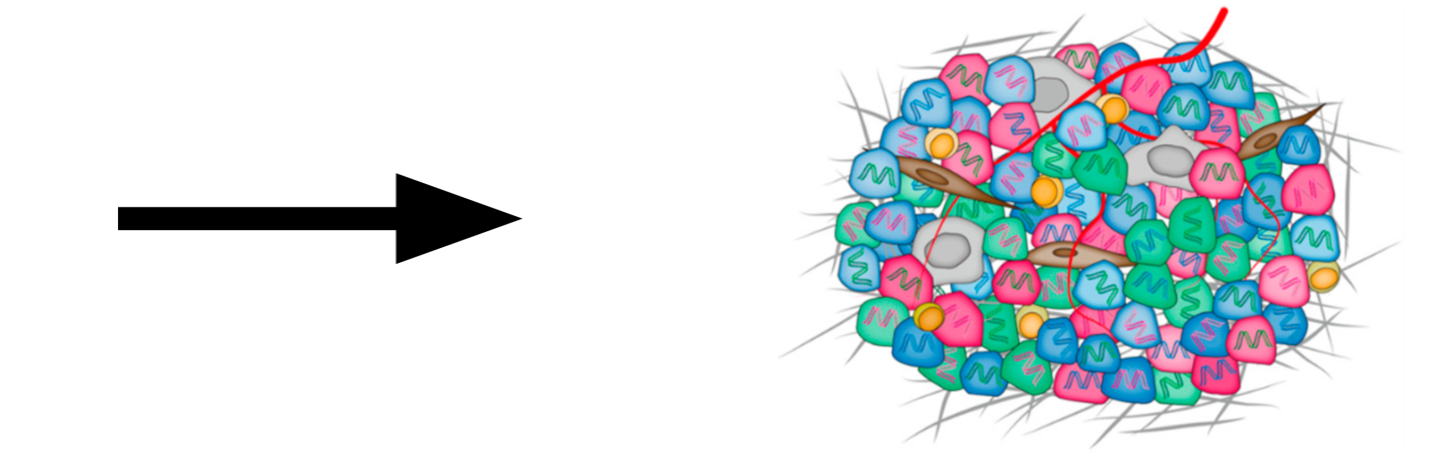
\includegraphics[width=4cm]{images/tumor_color_arrow.png}
      \end{figure}
    \end{column}
  \end{columns}
  % \end{overlayarea}
\end{frame}


\begin{frame}[t]{\textit{scRNA-seq}: Ventajas e inconvenientes}
  % \vskip0.2em
  % \begin{alertblock}{Comunidad}
  %   \vskip0.5mm
  %   Presencia de grupos de nodos que están
  %   más densamente conectados entre sí que con otros nodos.
  % \end{alertblock}
  \vskip-0.7cm
  \begin{columns}[t]
    \begin{column}{0.5\textwidth}
      \begin{alertblock}{Ventajas}
        \begin{itemize}
          \item Estatus funcional de cada célula.
          \item Caracterización de las poblaciones celulares. Potencial identificación de tipos celulares no esperados.
          \item Potencial aplicación traslacional: mejora del diagnóstico, terapias dirigidas, etc.
        \end{itemize}
      \end{alertblock}
    \end{column}
    \begin{column}{0.5\textwidth}
      \begin{alertblock}{Incovenientes}
        \begin{itemize}
          \item Altos costes económicos y protocolos complejos.
          \item No es práctica su aplicación en grandes cohortes de muestras.
          \item Baja eficiencia de captura de ARN.
          \item Mayor ruido técnico.
        \end{itemize}
      \end{alertblock}
    \end{column}
  \end{columns}
  \vskip0.5em
  \only<2,3,4>{\begin{beamercolorbox}[sep=0.2cm]{coloredboxstuff}
      \textbf{ Resultado:} \hspace{1.9cm}\textit{Bulk RNA-seq} sigue siendo el estándar. \hspace{\fill}
    \end{beamercolorbox}}
  \only<3,4>{\begin{beamercolorbox}[sep=0.2cm,center]{coloredboxstuff}
      \textbf{Problema:} No tiene en cuenta en qué proporción contribuye cada tipo celular a los niveles de expresión medidos.
    \end{beamercolorbox}}
  \only<4>{\begin{beamercolorbox}[sep=0.2cm,center]{coloredboxstuff}
      \textbf{Necesidad:} Métodos computacionales que permitan estimar las proporciones de cada tipo celular medidas en muestras \textit{bulk RNA-seq}.
    \end{beamercolorbox}}
\end{frame}

\subsection{1.3. Métodos de deconvolución de muestras \textit{bulk RNA-seq}}

\begin{frame}{Deconvolución de muestras \textit{bulk RNA-seq}}
  \alert{Deconvolución:} estimación de la señal individual de cada uno de los componentes (tipos celulares) a partir de una mezcla de los mismos (muestra tisular).
  \begin{itemize}
    \item Sustituto de experimentos \textit{scRNA-seq} por sus altos costes económicos o la imposibilidad de su aplicación.
    \item Control de la contribución de cada tipo celular a las muestras tisulares $\rightarrow$ evitar factores de confusión en análisis de expresión diferencial.
  \end{itemize}
  % \vskip-0.5em
  \begin{figure}
    \centering
    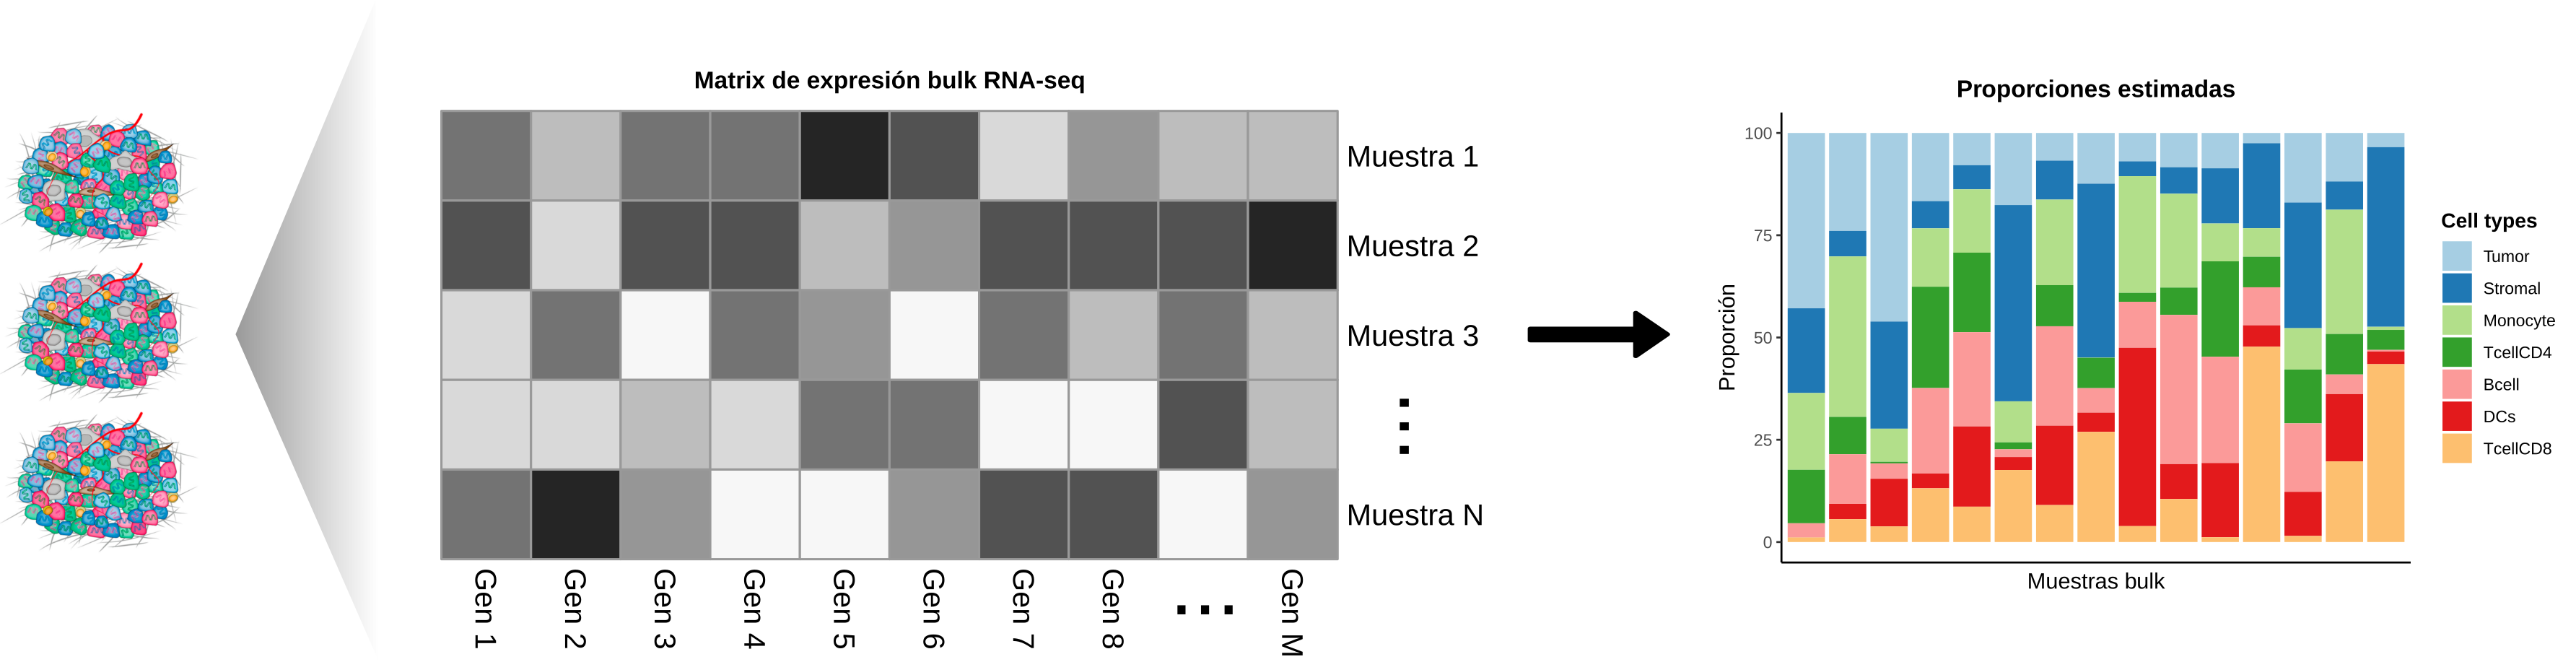
\includegraphics[width=14cm]{images/deconvolution_workflow.png}
  \end{figure}
\end{frame}


\begin{frame}{Deconvolución: marco de trabajo}
  \begin{overlayarea}{\linewidth}{1\textheight}
    % \vskip-1em

    \only<1>{
      \vskip0.7mm
      \hspace{-1mm}
      \begin{equation*}
        T_{ij} = \sum_{k=1}^K C_{ik} \cdot P_{kj} + e_{ij}
      \end{equation*}
    }
    \only<2>{
      \vskip0.15mm
      \centering
      \hspace{-4mm}
      \includegraphics[scale=0.135]{images/ecuación01_mod_def_def_1.png}
    }
    \only<3>{
      \vskip0.15mm
      \centering
      \hspace{-5.2mm}
      \includegraphics[scale=0.135]{images/ecuación01_mod_def_def_2.png}
    }
    \only<4>{
      \vskip0.15mm
      \centering
      \hspace{-6.4mm}
      \includegraphics[scale=0.135]{images/ecuación01_mod_def_def_3.png}
    }
    \vskip3mm
    \begin{columns}
      \begin{column}{0.5\textwidth}
        \only<1>{
          \vskip2.25mm
          \centering
          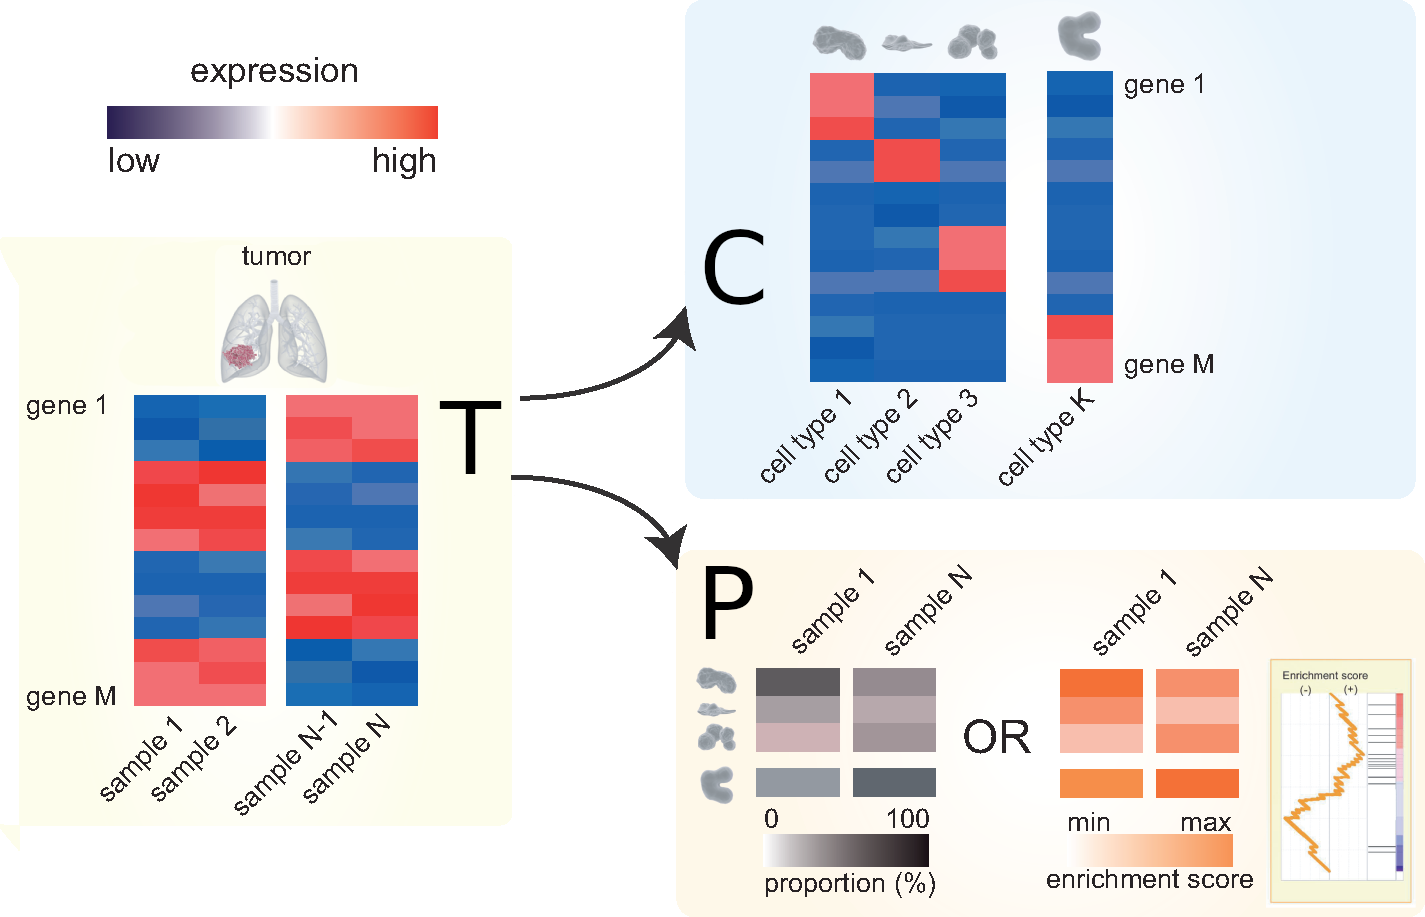
\includegraphics[width=8.5cm]{images/figure4.png}
        }
        \only<2>{
          \vskip-1em
          \centering
          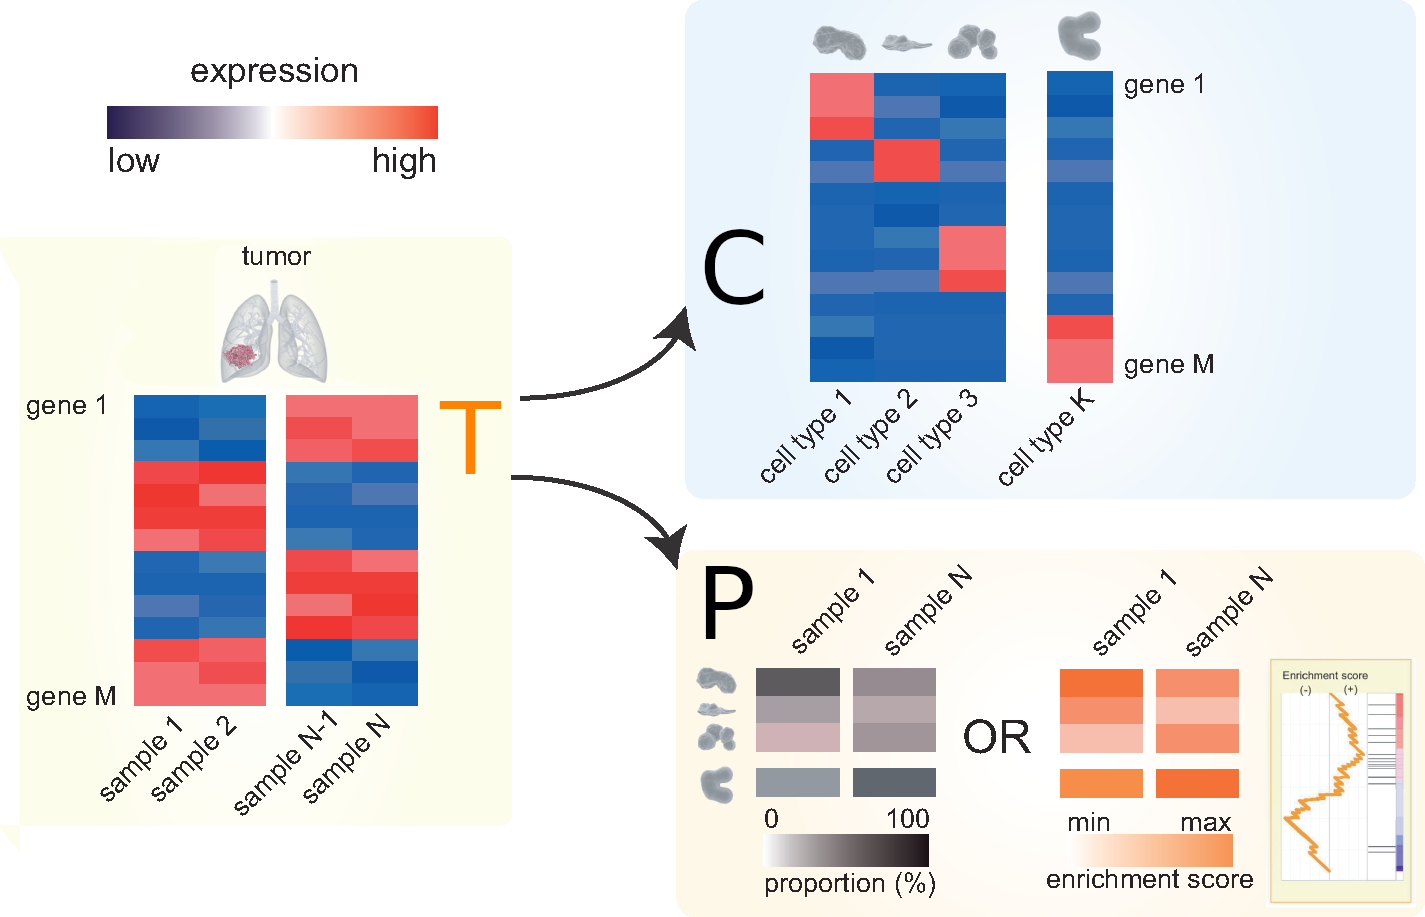
\includegraphics[width=8.5cm]{images/expression_deconv_1.png}
        }
        \only<3>{
          \vskip-1em
          \centering
          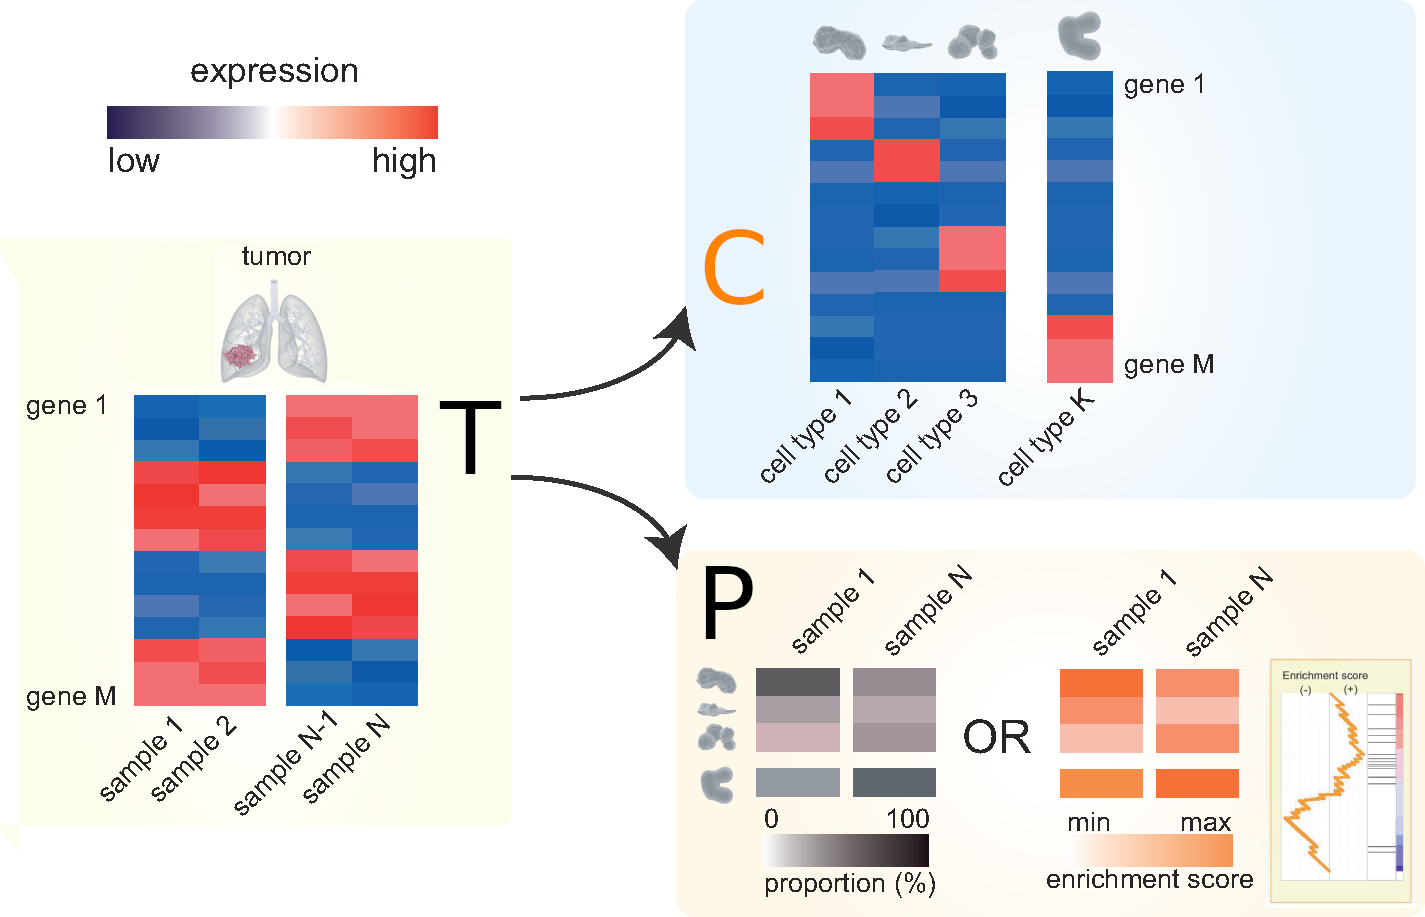
\includegraphics[width=8.5cm]{images/expression_deconv_2.png}
        }
        \only<4>{
          \vskip-1em
          \centering
          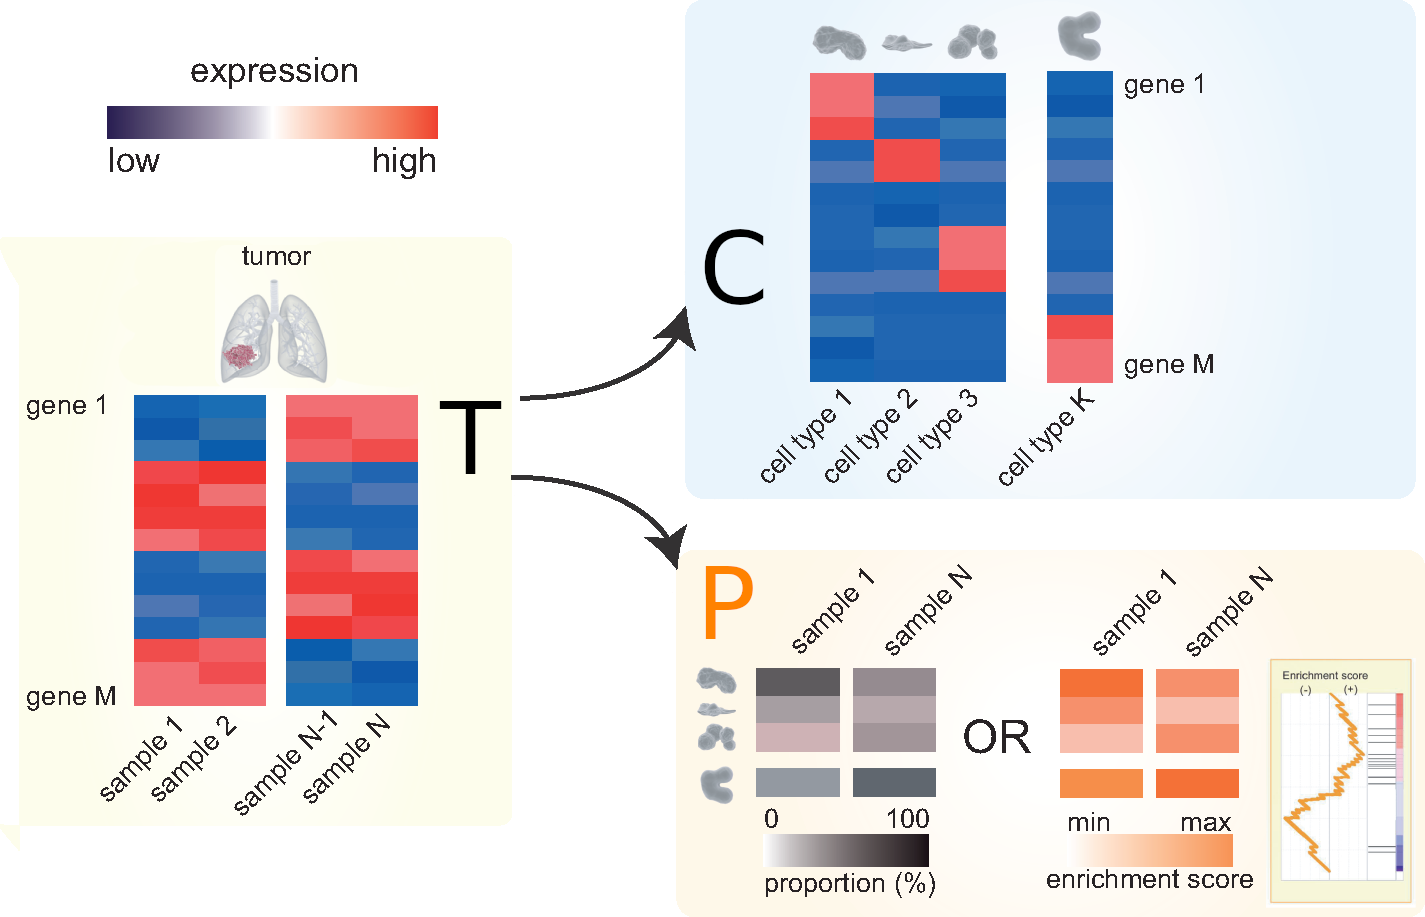
\includegraphics[width=8.5cm]{images/expression_deconv_3.png}
        }
      \end{column}

      \begin{column}{0.4\textwidth}
        \begin{textblock*}{6cm}(10cm,3.5cm)
          \begin{itemize}
            \item $i$: genes ($i = 1...M$).
            \item $j$: muestras \textit{bulk} ($j = 1...N$).
            \item $k$: tipos celulares ($k = 1...K$).
          \end{itemize}
        \end{textblock*}

        \only<4>{
          \begin{textblock*}{6cm}(10cm,5.5cm)
            \begin{alertblock}{Herramientas publicadas}
              \begin{itemize}
                \item Enriquecimiento de sets de genes.
                \item Mínimos cuadrados ordinarios.
                \item $\upsilon$-SVR
              \end{itemize}
            \end{alertblock}
          \end{textblock*}
        }
      \end{column}
    \end{columns}

  \end{overlayarea}
\end{frame}

\begin{frame}[fragile]{Método de deconvolución digitalDLSorter}
  \begin{alertblock}{Características}
    \begin{itemize}
      \item Método basado en \alert{Aprendizaje Profundo} $\rightarrow$ revolución en el campo del Aprendizaje Automático durante los últimos años por su desempeño.
      \item Uso de datos \alert{\textit{scRNA-seq}} $\rightarrow$ perfiles de expresión procedentes del propio entorno de estudio (micro-entorno tumoral cáncer de mama, cáncer de colon, entorno neuronal, etc.).
    \end{itemize}
  \end{alertblock}

  \begin{alertblock}{Implementación}
    \begin{itemize}
      \item \textit{Pipeline} escrita en varios lenguajes de programación.
      \item Cada paso escribe los datos intermedios en disco como ficheros tabulados.
      \item No ofrece la opción de utilizar modelos preentrenados.
      \item Uso complicado por otros usuarios.
    \end{itemize}
  \end{alertblock}
\end{frame}


%--------------------------------------------------------------------------%

%%%%%%%%%%%%%%%%%%%%%%%%%%%%%%%%%%%%%%%%%%%%%%%%%%%%%%%%%%%%%%%%%%%%%%%%%%%%%%%%%%%%
%%%%%%%%%%%%%%%%%%%%%%%%%%%%%%%%%%% OBJETIVOS %%%%%%%%%%%%%%%%%%%%%%%%%%%%%%%%%%%%%%
%%%%%%%%%%%%%%%%%%%%%%%%%%%%%%%%%%%%%%%%%%%%%%%%%%%%%%%%%%%%%%%%%%%%%%%%%%%%%%%%%%%%

\section[Objetivos]{Objetivos}

\begin{frame}{Objetivos}
  % \metroset{block=fill}
  % \vskip-1em
  % \begin{alertblock}{Objetivos}
  %   \vskip0.20em
  %   Grafo ponderado con pesos basados en el número de vecinos que comparten.
  % \end{alertblock}
  \begin{enumerate}[<alert@+>]
    \item Transformación de la \textit{pipeline} original en un paquete de R.
          \begin{itemize}
            \item Unificación de los lenguajes de programación $\rightarrow$ R.
            \item Evitar la lectura/escritura de ficheros tabulados en disco.
            \item Funcionalidades nuevas $\rightarrow$ uso de ficheros HDF5 como \textit{back-end}, implementación de parámetros para construir modelos más personalizados.
            \item Generación de documentación y viñeta $\rightarrow$ facilitar su uso.
          \end{itemize}
    \item Análisis de datos \textit{scRNA-seq} procedentes de cáncer de mama.
          \begin{itemize}
            \item Separación tipos tumorales y no tumorales.
            \item Identificación de tipos celulares no tumorales.
          \end{itemize}
    \item Aplicación de la herramienta implementada.
          \begin{itemize}
            \item Construcción de varios modelos y comparativa.
            \item Incorporación de los mejores como modelos preentrenados en el paquete.
          \end{itemize}
  \end{enumerate}

\end{frame}

%%%%%%%%%%%%%%%%%%%%%%%%%%%%%%%%%%%%%%%%%%%%%%%%%%%%%%%%%%%%%%%%%%%%%%%%%%%%%%%%%%%%
%%%%%%%%%%%%%%%%%%%%%%%%%%%%%%%%%%%%% PAQUETE R %%%%%%%%%%%%%%%%%%%%%%%%%%%%%%%%%%%%
%%%%%%%%%%%%%%%%%%%%%%%%%%%%%%%%%%%%%%%%%%%%%%%%%%%%%%%%%%%%%%%%%%%%%%%%%%%%%%%%%%%%

\section[digitalDLSorteR: transformación de la \textit{pipeline} en paquete de R]{digitalDLSorteR: transformación de la \textit{pipeline} en paquete de R}

% Fundamento -----------------------------------------------------------------

\subsection{2.1. Fundamento del método}

\begin{frame}[fragile]{Fundamento del método}
  \begin{overlayarea}{\linewidth}{1\textheight}
    \only<1>{
      \centering
      \vskip1em
      \hspace{-2.8mm}
      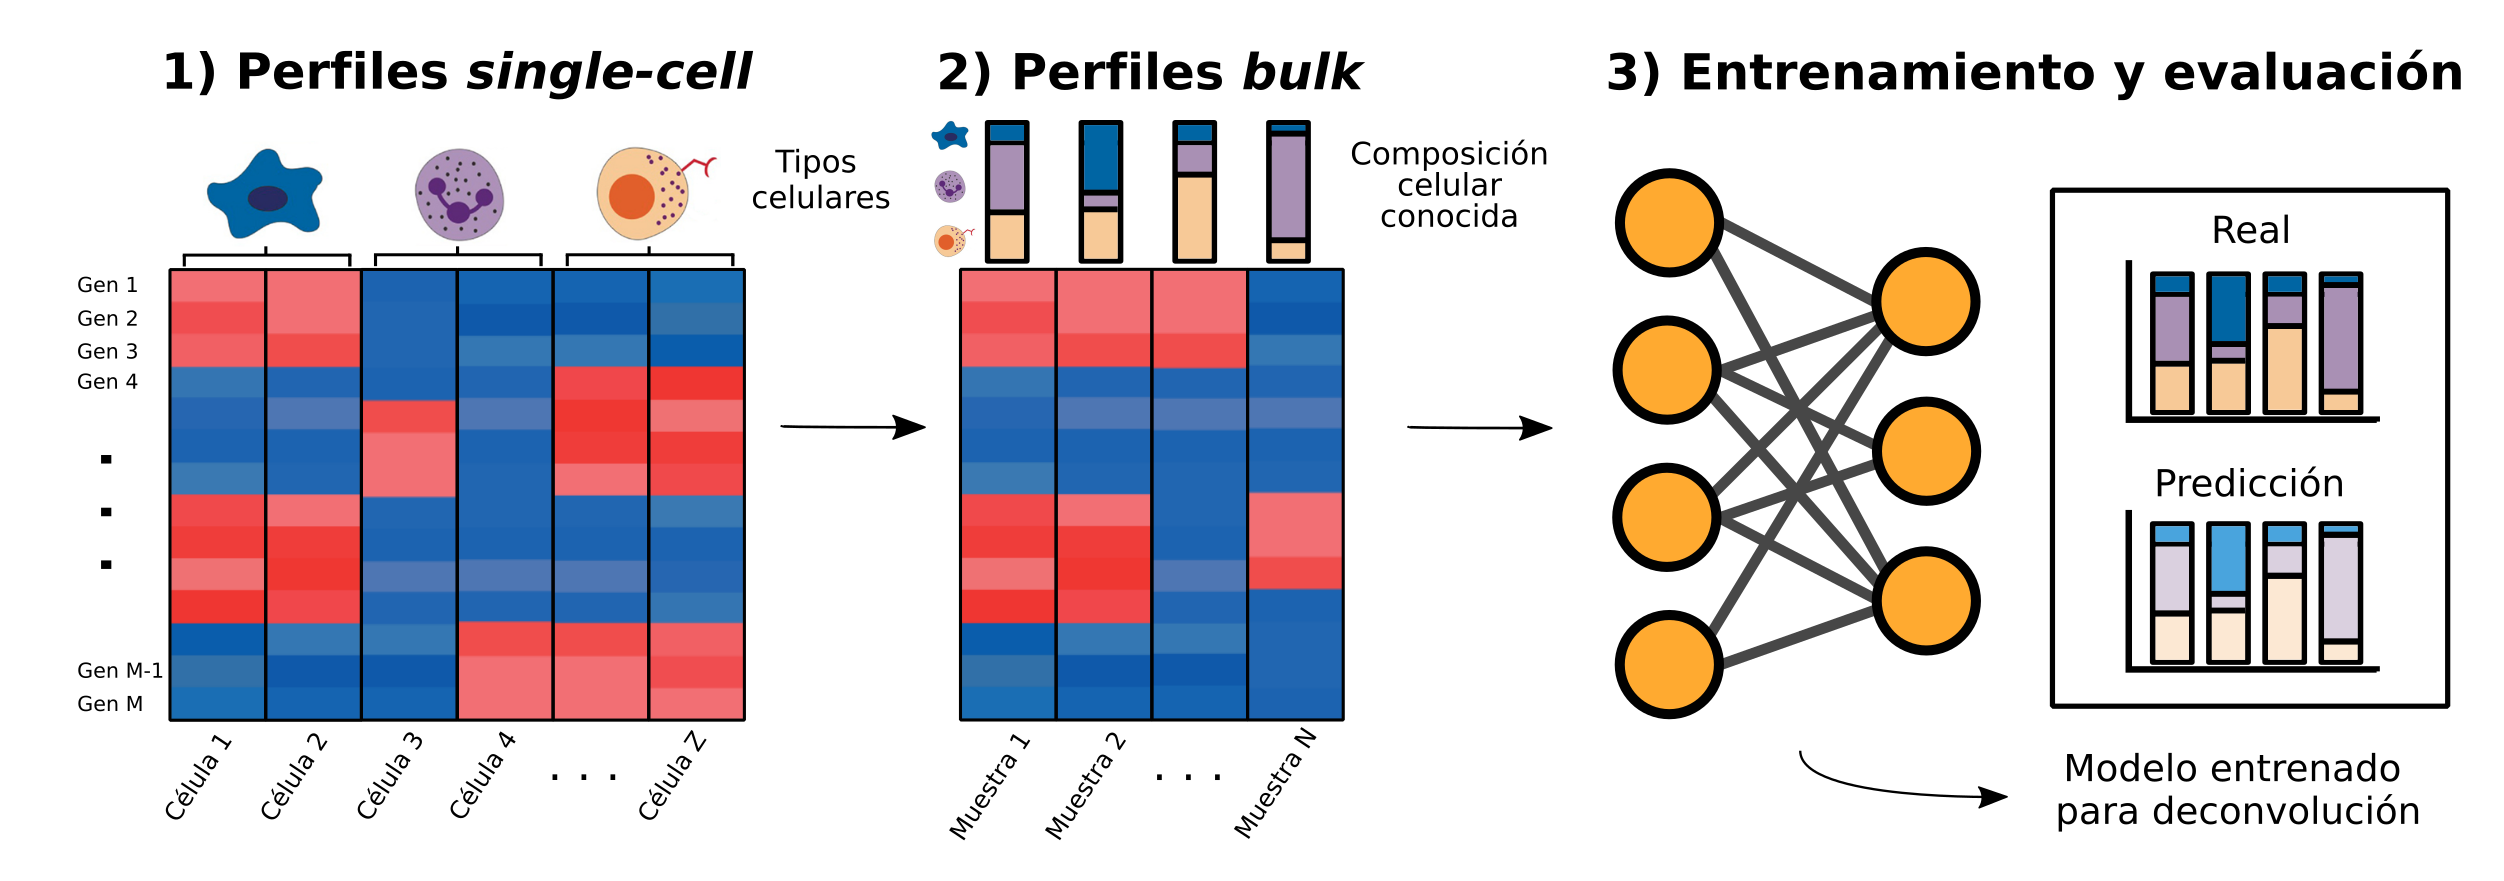
\includegraphics[width=10cm]{images/fund_model_0.png}
    }
    \only<2>{
      \centering
      \vskip1em
      \hspace{-4mm}
      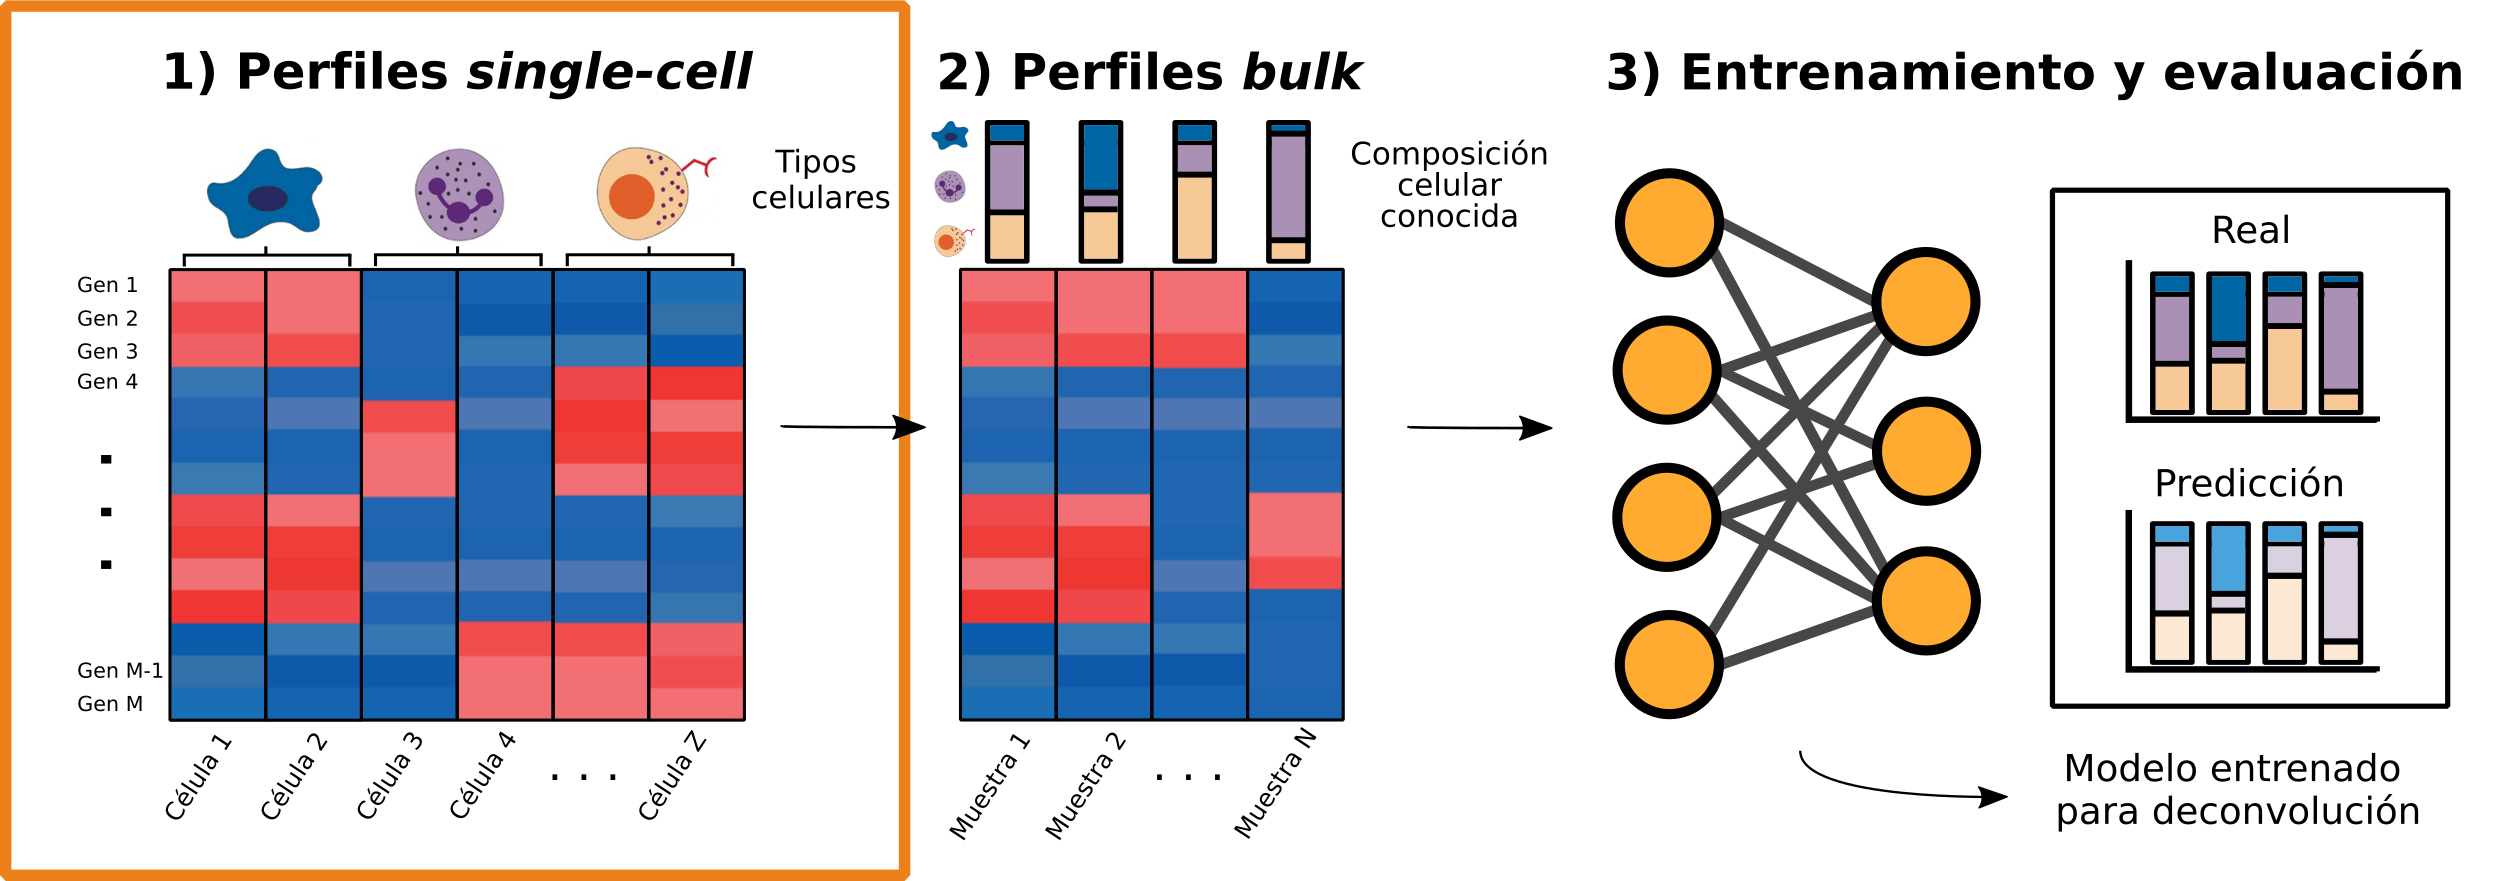
\includegraphics[width=10cm]{images/fund_model_1.png}
    }
    \only<3>{
      \centering
      \vskip1em
      \hspace{-5.2mm}
      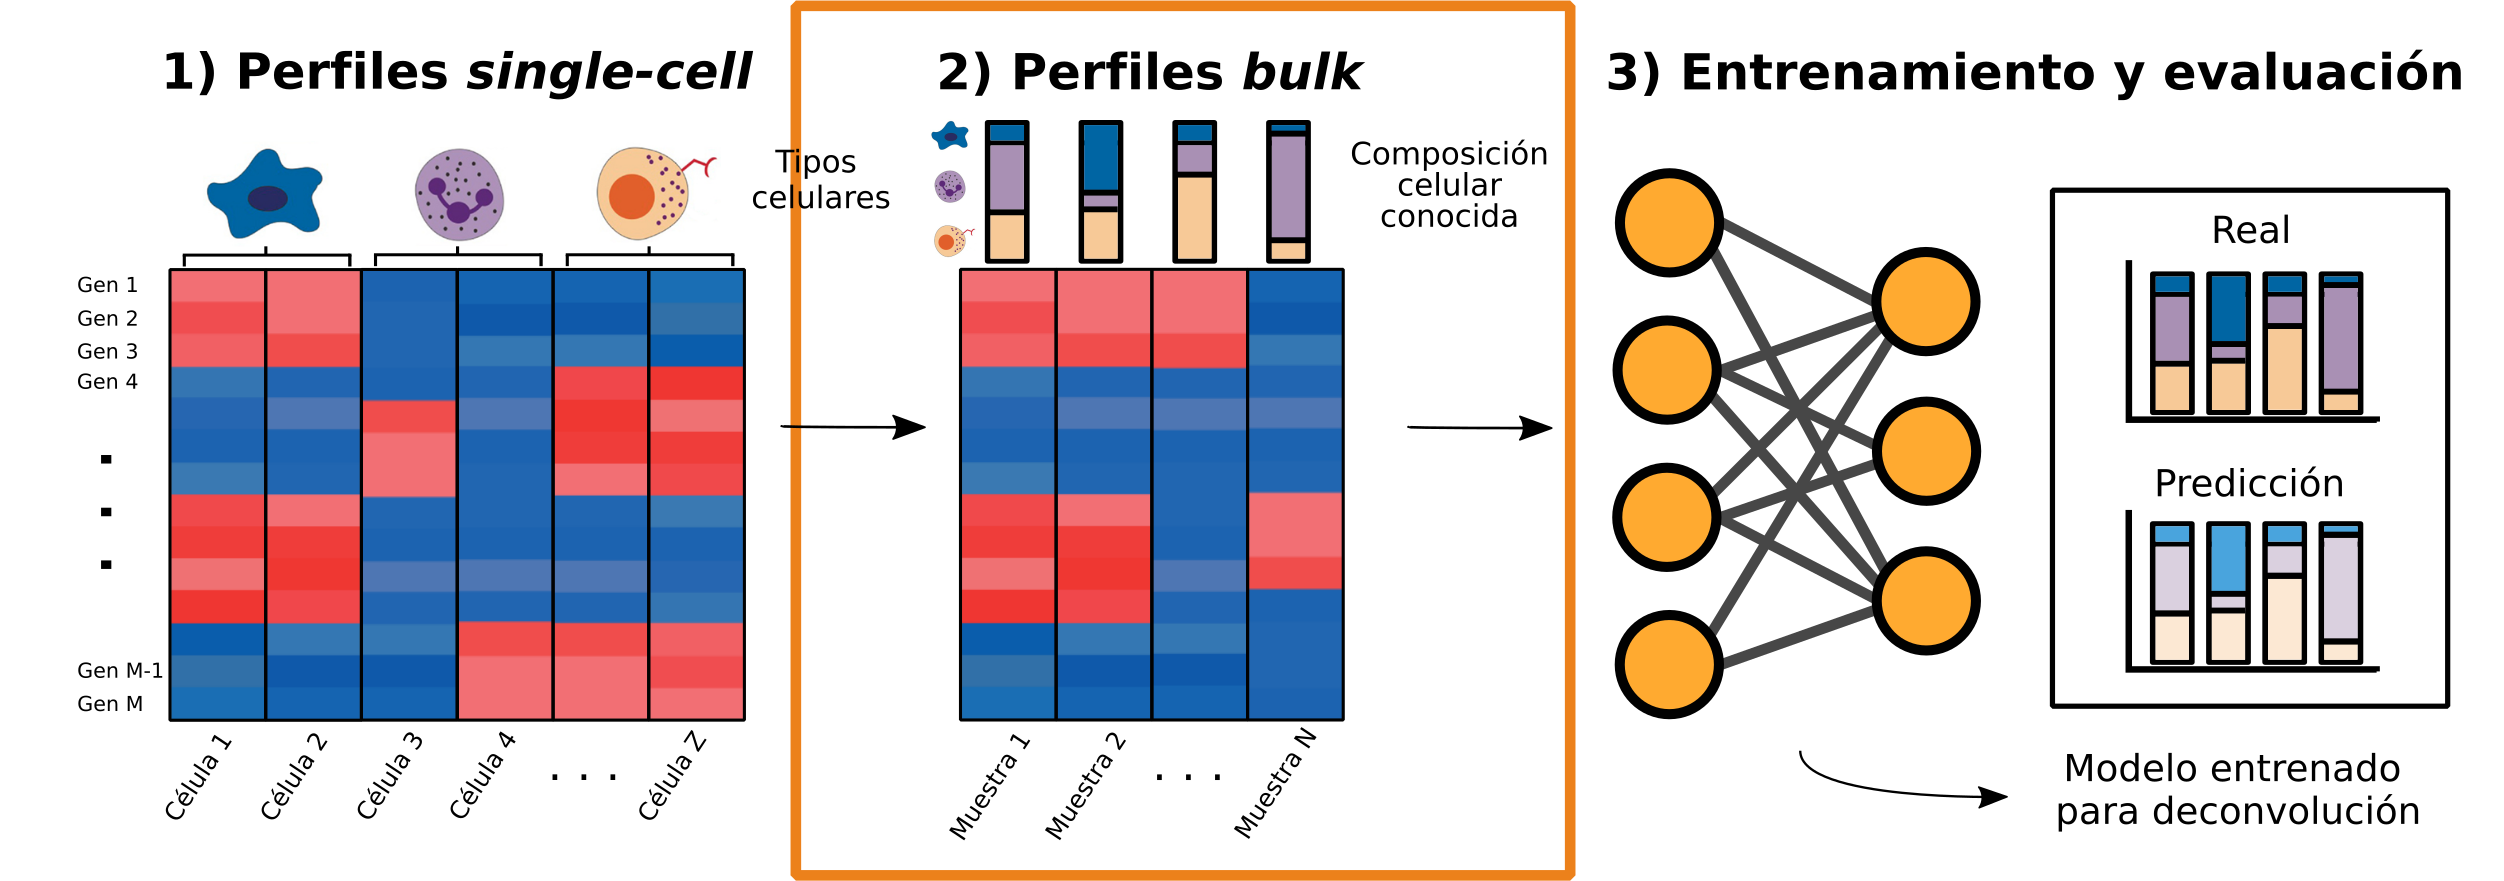
\includegraphics[width=10cm]{images/fund_model_2.png}
    }
    \only<4>{
      \centering
      \vskip1em
      \hspace{-6.4mm}
      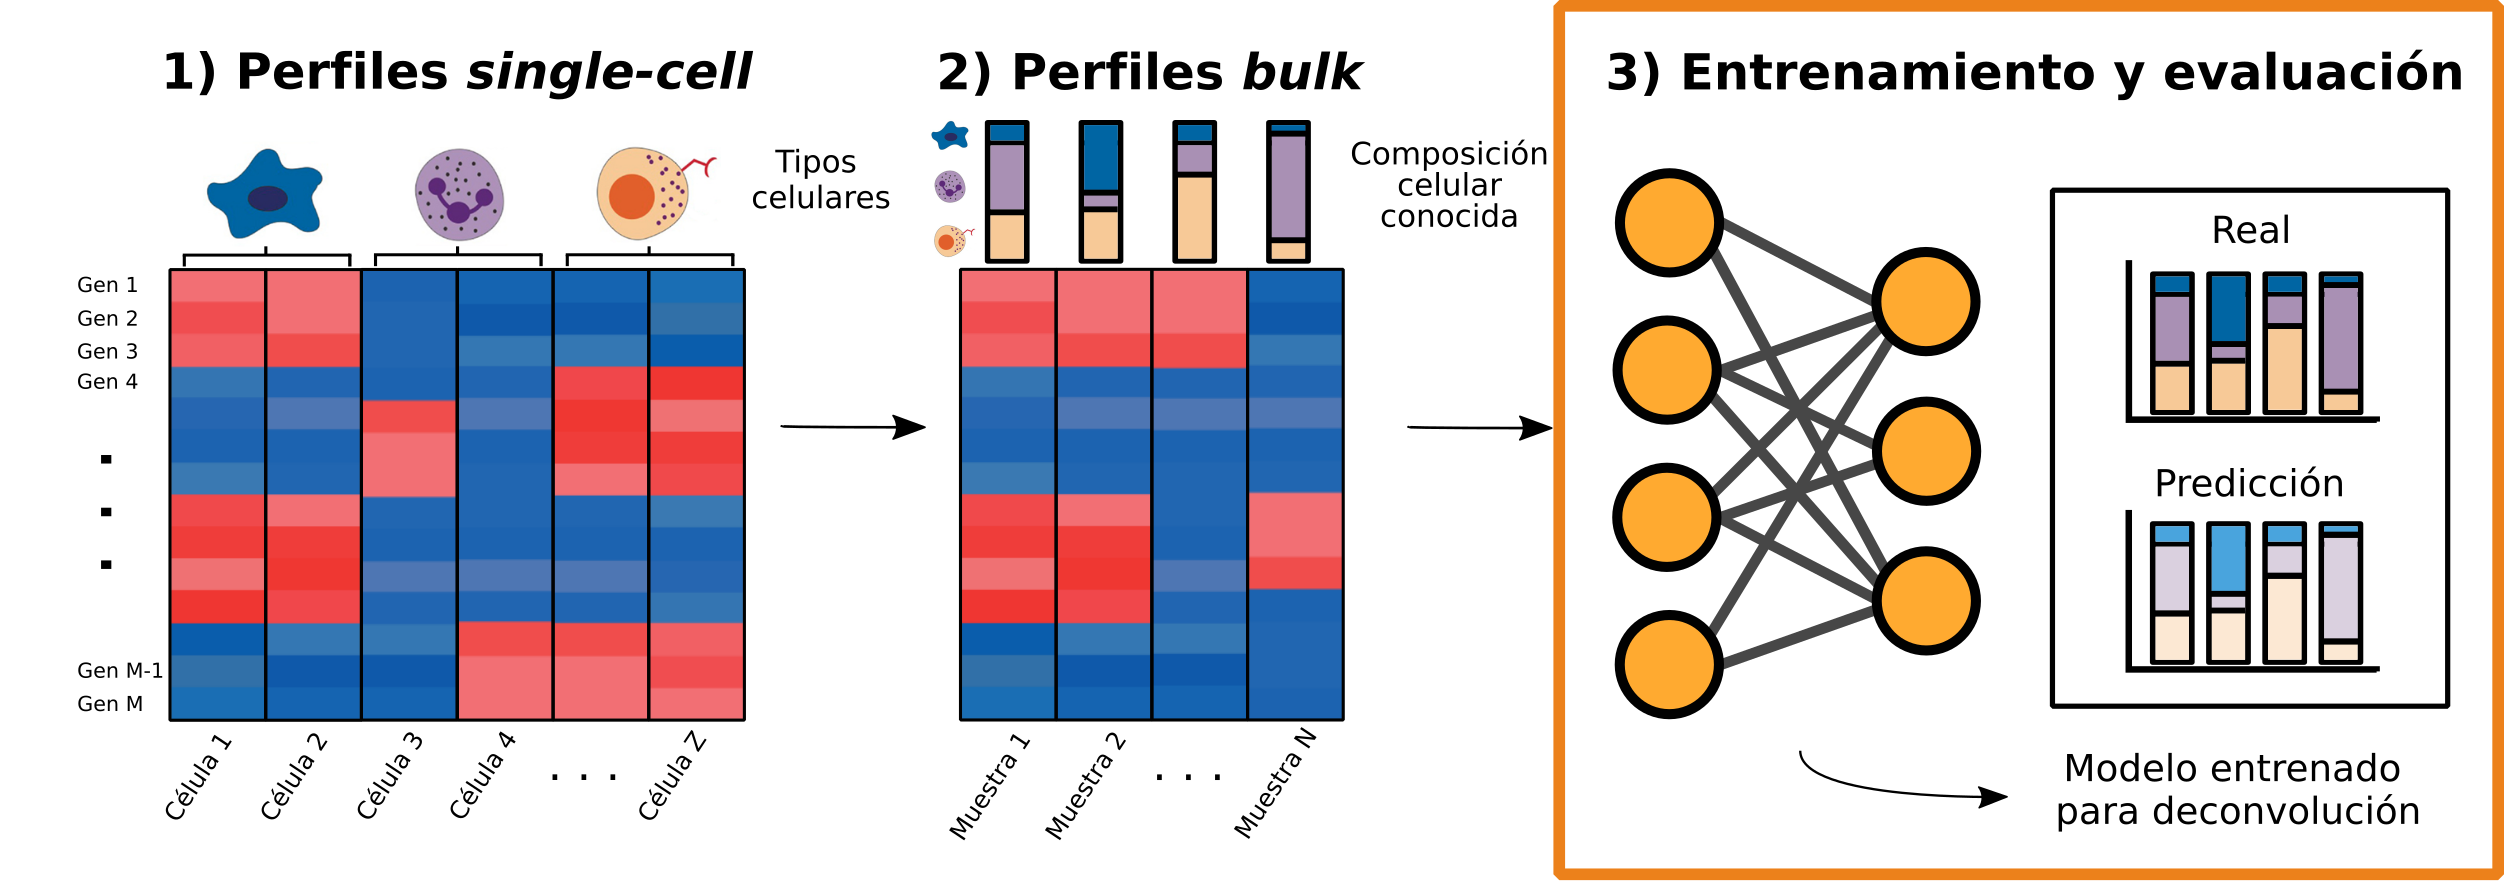
\includegraphics[width=10cm]{images/fund_model_3.png}
    }

    \only<5>{
      \centering
      \vskip1em
      \includegraphics[scale=0.2]{images/ecuación01_mod_def_def_3.png}
      \vskip1.55em
    }

    \begin{enumerate}
      \alert<2>{\item Simulación de perfiles \textit{scRNA-seq} (si es necesario):} uso del modelo ZINB-WaVE en caso de tipos celulares poco representados o pocas células de partida.
            \alert<3>{\item Simulación de perfiles \textit{bulk RNA-seq} de composición celular conocida}: agregación de perfiles \textit{single-cell} en función del tipo celular al que pertenecen.
            \alert<4>{\item Entrenamiento y evaluación de la Red Neuronal Profunda}: deconvolución de nuevas muestras \textit{bulk}.
    \end{enumerate}
  \end{overlayarea}
\end{frame}

% Herramienta -----------------------------------------------------------------

\subsection{2.1. digitalDLSorteR: flujo de trabajo}

\begin{frame}{digitalDLSorteR: flujo de trabajo}

  \begin{alertblock}{Objetivo del método como paquete}
    \begin{enumerate}
      \item Permitir la deconvolución directa de muestras \textit{bulk RNA-seq}.
      \item Permitir la construcción de nuevos modelos a partir de datos \textit{scRNA-seq}
    \end{enumerate}
  \end{alertblock}

  \begin{center}
    \begin{tikzpicture}[sibling distance=5.5cm, level distance=2cm,
        edge from parent/.style={draw,Orange,ultra thick},
        every node/.style = {align=center}]]
      \node[draw=none,fill=none] {\Large{\alert{\textbf{digitalDLSorteR ofrece }}} \\ \Large{\alert{\textbf{dos flujos de trabajo}}}}
      child { node {1. Uso de modelos preentrenados\\integrados en el paquete} }
      child { node {2. Construcción de nuevos modelos\\a partir de \textit{scRNA-seq}} };
    \end{tikzpicture}
  \end{center}
\end{frame}


% Modelos preentrenados ----------------------------------------------------------
% \hbox{\hspace{-0.5em}
\begin{frame}[fragile]
  \frametitle{Uso de modelos preentrenados}
  \begin{figure}
    \centering
    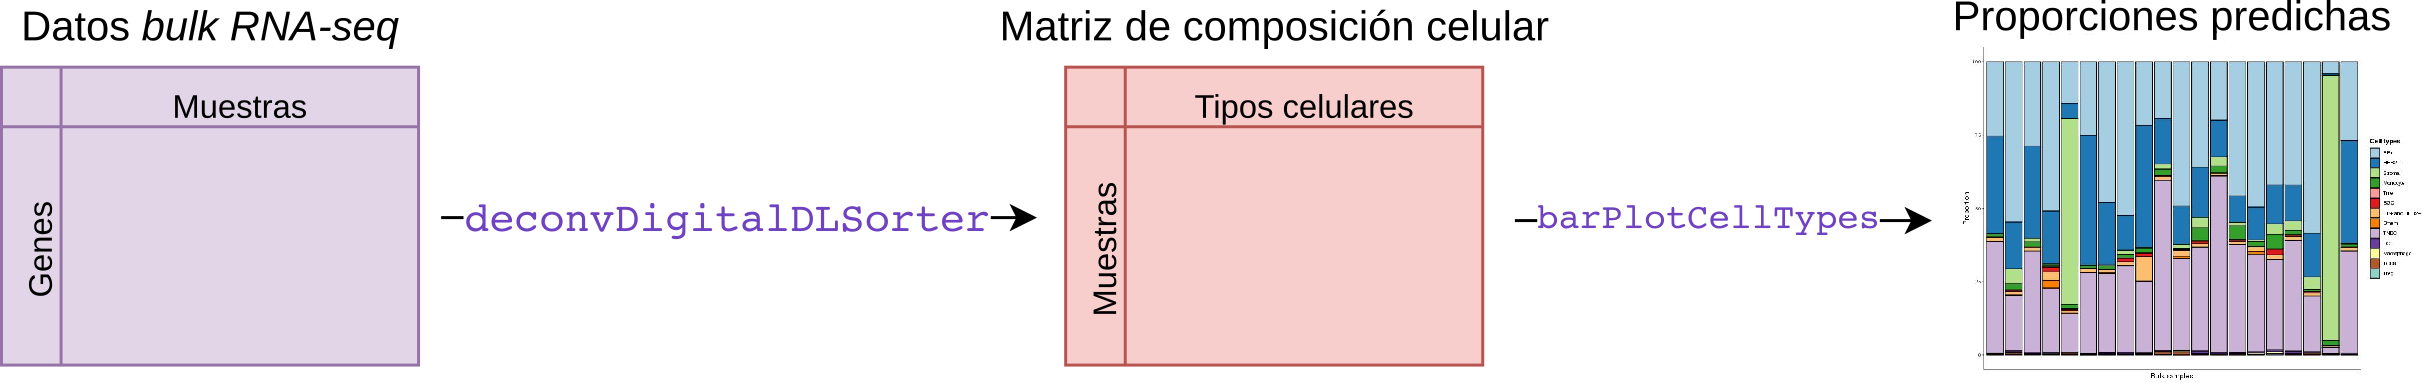
\includegraphics[width=13cm]{images/modelo_preentrenado_3.png}
  \end{figure}

  \begin{columns}
    \begin{column}{0.45\textwidth}
      \lstinputlisting[]{./boxcodes/boxcode1.R}
    \end{column}

    \begin{column}{0.6\textwidth}
      \begin{itemize}
        \item Modelos para la cuantificación de células inmunes en cáncer de mama.
              \begin{enumerate}
                \item Modelo genérico: 7 tipos celulares.
                \item Modelo específico: 13 tipos celulares.
              \end{enumerate}
        \item Datos procedentes de Chung et al., 2017 (\href{https://www.ncbi.nlm.nih.gov/geo/query/acc.cgi?acc=GSE75688}{GSE75688}).
      \end{itemize}
    \end{column}
  \end{columns}
\end{frame}


% Construcción de nuevos modelos --------------------------------------------------

\begin{frame}{Construcción de nuevos modelos}
  \begin{alertblock}{Clases}
    \begin{itemize}
      \item \textit{DigitalDLSorter}: núcleo del paquete. 
      \item \textit{ProbMatrixCellTypes}: información relativa a las matrices de composición celular. 
      \item \textit{DigitalDLSorterDNN}: información relativa a la Red Neuronal Profunda.
      \item Otras clases: \textit{SingleCellExperiment}, \textit{SummarizedExperiment}, etc.
    \end{itemize}
  \end{alertblock}

  \begin{alertblock}{Flujo de trabajo}
    \begin{enumerate}
      \item Carga de datos y simulación de nuevos perfiles \textit{single-cell} (si es necesario).
      \item Generación de matrices de composición celular.
      \item Simulación de perfiles \textit{bulk RNA-seq} de acuerdo a las proporciones establecidas en el paso anterior. Preparación de los datos para el entrenamiento.
      \item Entrenamiento de la red neuronal y evaluación. 
      \item Carga de nuevos datos y su deconvolución.
    \end{enumerate}
  \end{alertblock}
\end{frame}

% Carga de datos y simulación de perfiles single-cell -------------------------------

\begin{frame}[fragile]
  \frametitle{1. Carga de datos y simulación de perfiles \textit{single-cell}}

  \begin{figure}
    \centering
    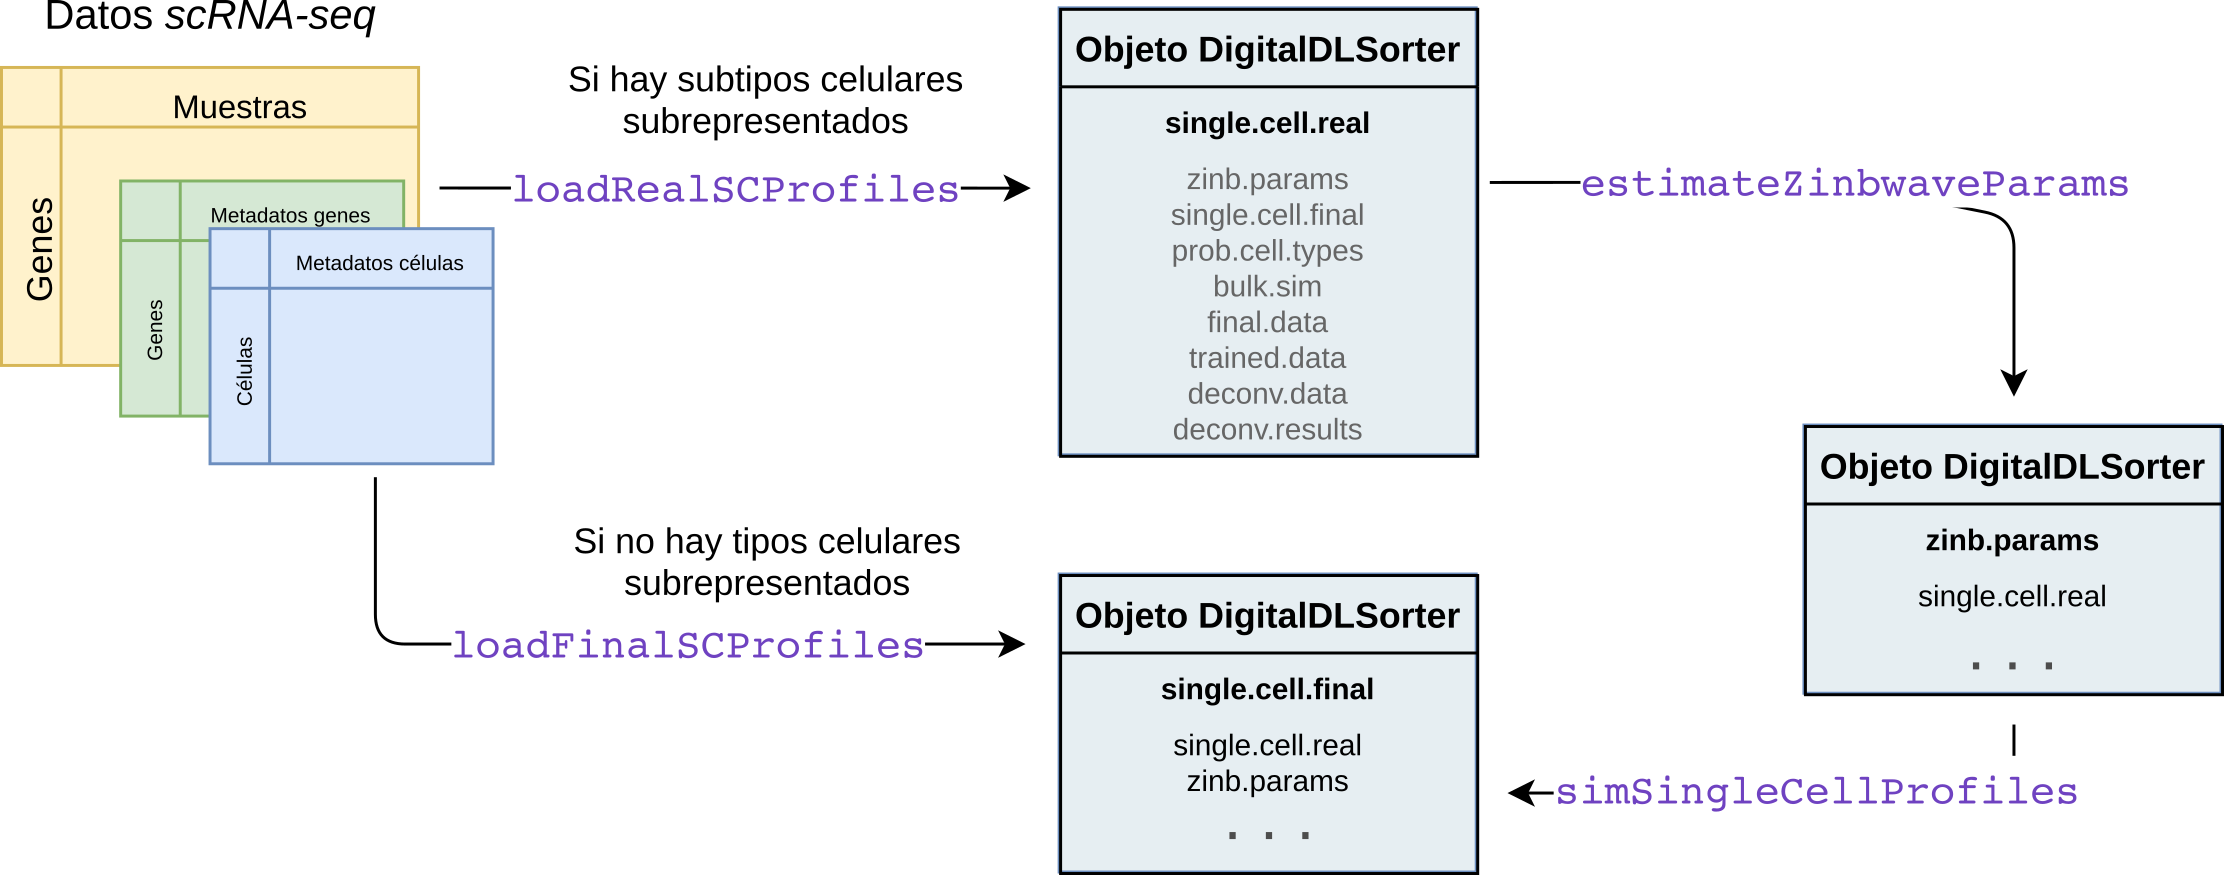
\includegraphics[width=11cm]{images/load_data_1.png}
  \end{figure}

  \begin{itemize}
    \item Carga de los datos en un objeto de la clase \textit{DigitalDLSorter} $\rightarrow$ matriz de expresión, metadatos de células y metadatos de genes.
    \item Si es necesario: estimación de parámetros mediante el modelo ZINB-WaVE y simulación de nuevos perfiles \textit{single-cell}: distribución binomial negativa cero inflada.
  \end{itemize}
\end{frame}

\begin{frame}[fragile,t]{1. Carga de datos y simulación de perfiles \textit{single-cell}}
  \begin{columns}
    \begin{column}{0.5\textwidth}
      \lstinputlisting[basicstyle=\fontsize{7}{8.4}\ttfamily]{./boxcodes/boxcode2.R}
    \end{column}
    % \hspace{0.5cm}
    \begin{column}{0.5\textwidth}
      \lstinputlisting[basicstyle=\fontsize{7}{8.4}\ttfamily]{./boxcodes/boxcode3.R}
    \end{column}
  \end{columns}
\end{frame}

% Generación de matrices de composición celular ---------------------------------

\begin{frame}[fragile]{2. Generación de la matriz de composición celular}

  \begin{figure}
    \centering
    
\includegraphics[width=12cm]{images/generateBulkMatrix.png}
  \end{figure}

  \begin{itemize}
    \item Carga de los datos en un objeto de la clase \textit{DigitalDLSorter} $\rightarrow$ matriz de expresión, metadatos de células y metadatos de genes.
    \item Si es necesario: estimación de parámetros mediante el modelo ZINB-WaVE y simulación de nuevos perfiles \textit{single-cell}: distribución binomial negativa cero inflada.
  \end{itemize}
\end{frame}


%%%%%%%%%%%%%%%%%%%%%%%%%%%%%%%%%%%%%%%%%%%%%%%%%%%%%%%%%%%%%%%%%%%%%%%%%%%%%%%%%%%%
%%%%%%%%%%%%%%%%%%%%%%%%%%%%%%%%%%%%% ANÁLISIS %%%%%%%%%%%%%%%%%%%%%%%%%%%%%%%%%%%%%
%%%%%%%%%%%%%%%%%%%%%%%%%%%%%%%%%%%%%%%%%%%%%%%%%%%%%%%%%%%%%%%%%%%%%%%%%%%%%%%%%%%%





%%%%%%%%%%%%%%%%%%%%%%%%%%%%%%%%%%%%%%%%%%%%%%%%%%%%%%%%%%%%%%%%%%%%%%%%%%%%%%%%%%%%
%%%%%%%%%%%%%%%%%%%%%%%%%%%%%%%%%%%%%% MODELOS %%%%%%%%%%%%%%%%%%%%%%%%%%%%%%%%%%%%%
%%%%%%%%%%%%%%%%%%%%%%%%%%%%%%%%%%%%%%%%%%%%%%%%%%%%%%%%%%%%%%%%%%%%%%%%%%%%%%%%%%%%



%--------------------------------------------------------------------------%

\begin{frame}{Introducción: Clustering}
  \vskip1em
  Conocer la \alert{\textbf{estructura de las poblaciones celulares}}.
  \Fontvi
  \vskip0.5em
  \begin{columns}
    \begin{column}{0.5\textwidth}
      \begin{alertblock}{Por qué}
        \begin{itemize}
          \item Qué fenotipos hay presentes.
          \item Qué perfiles de expresión.
          \item Qué células son similares y qué celulas no.
        \end{itemize}
      \end{alertblock}
      \begin{alertblock}{Características}
        \begin{itemize}
          \item Escalable.
          \item No paraḿetrico.
          \item Alta dimensionalidad.
          \item Geometrías no estándar.
        \end{itemize}
      \end{alertblock}
    \end{column}
    \begin{column}{0.4\textwidth}
      \begin{textblock*}{5cm}(7cm,3cm)
        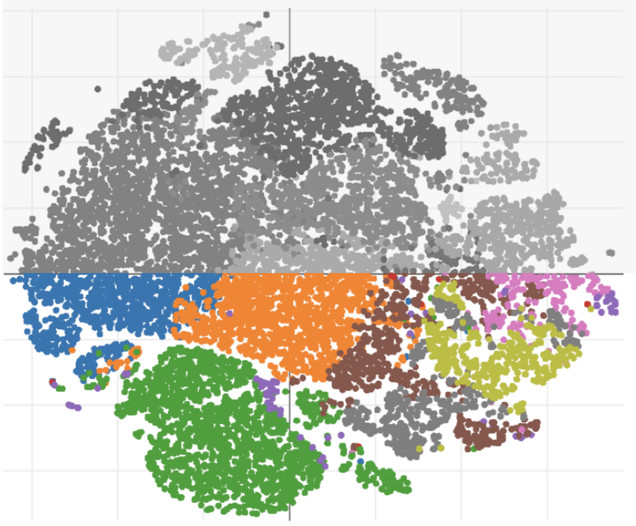
\includegraphics[scale=.5]{images/10x_mod.jpg}
      \end{textblock*}
    \end{column}
  \end{columns}

  \begin{center}
    \fontsize{15}{7.2}\selectfont
    \begin{itemize}
      \begin{center}
        \vskip1em
        \hskip-12mm
        \item<2>[\alert{\textbf{PhenoGraph}}]
      \end{center}
    \end{itemize}
    % \alert{\textbf{PhenoGraph}}  
  \end{center}
\end{frame}

%--------------------------------------------------------------------------%


\section{PhenoGraph}

\begin{frame}{PhenoGraph}
  \alert{Aprendizaje no supervisado:}
  Agrupa $N$ células individuales en subpoblaciones (clústers) que representan los fenotipos
  presentes en la muestra.
  \begin{itemize}
    \item Input: matriz $N$x$D$.
    \item Busca regiones densas en el espacio $D$-dimensional $\rightarrow$ grafo.
    \item Busca comunidades en el grafo.
    \item Output: index asignando cada célula a una subpoblación.
  \end{itemize}
  \vskip-0.5em
  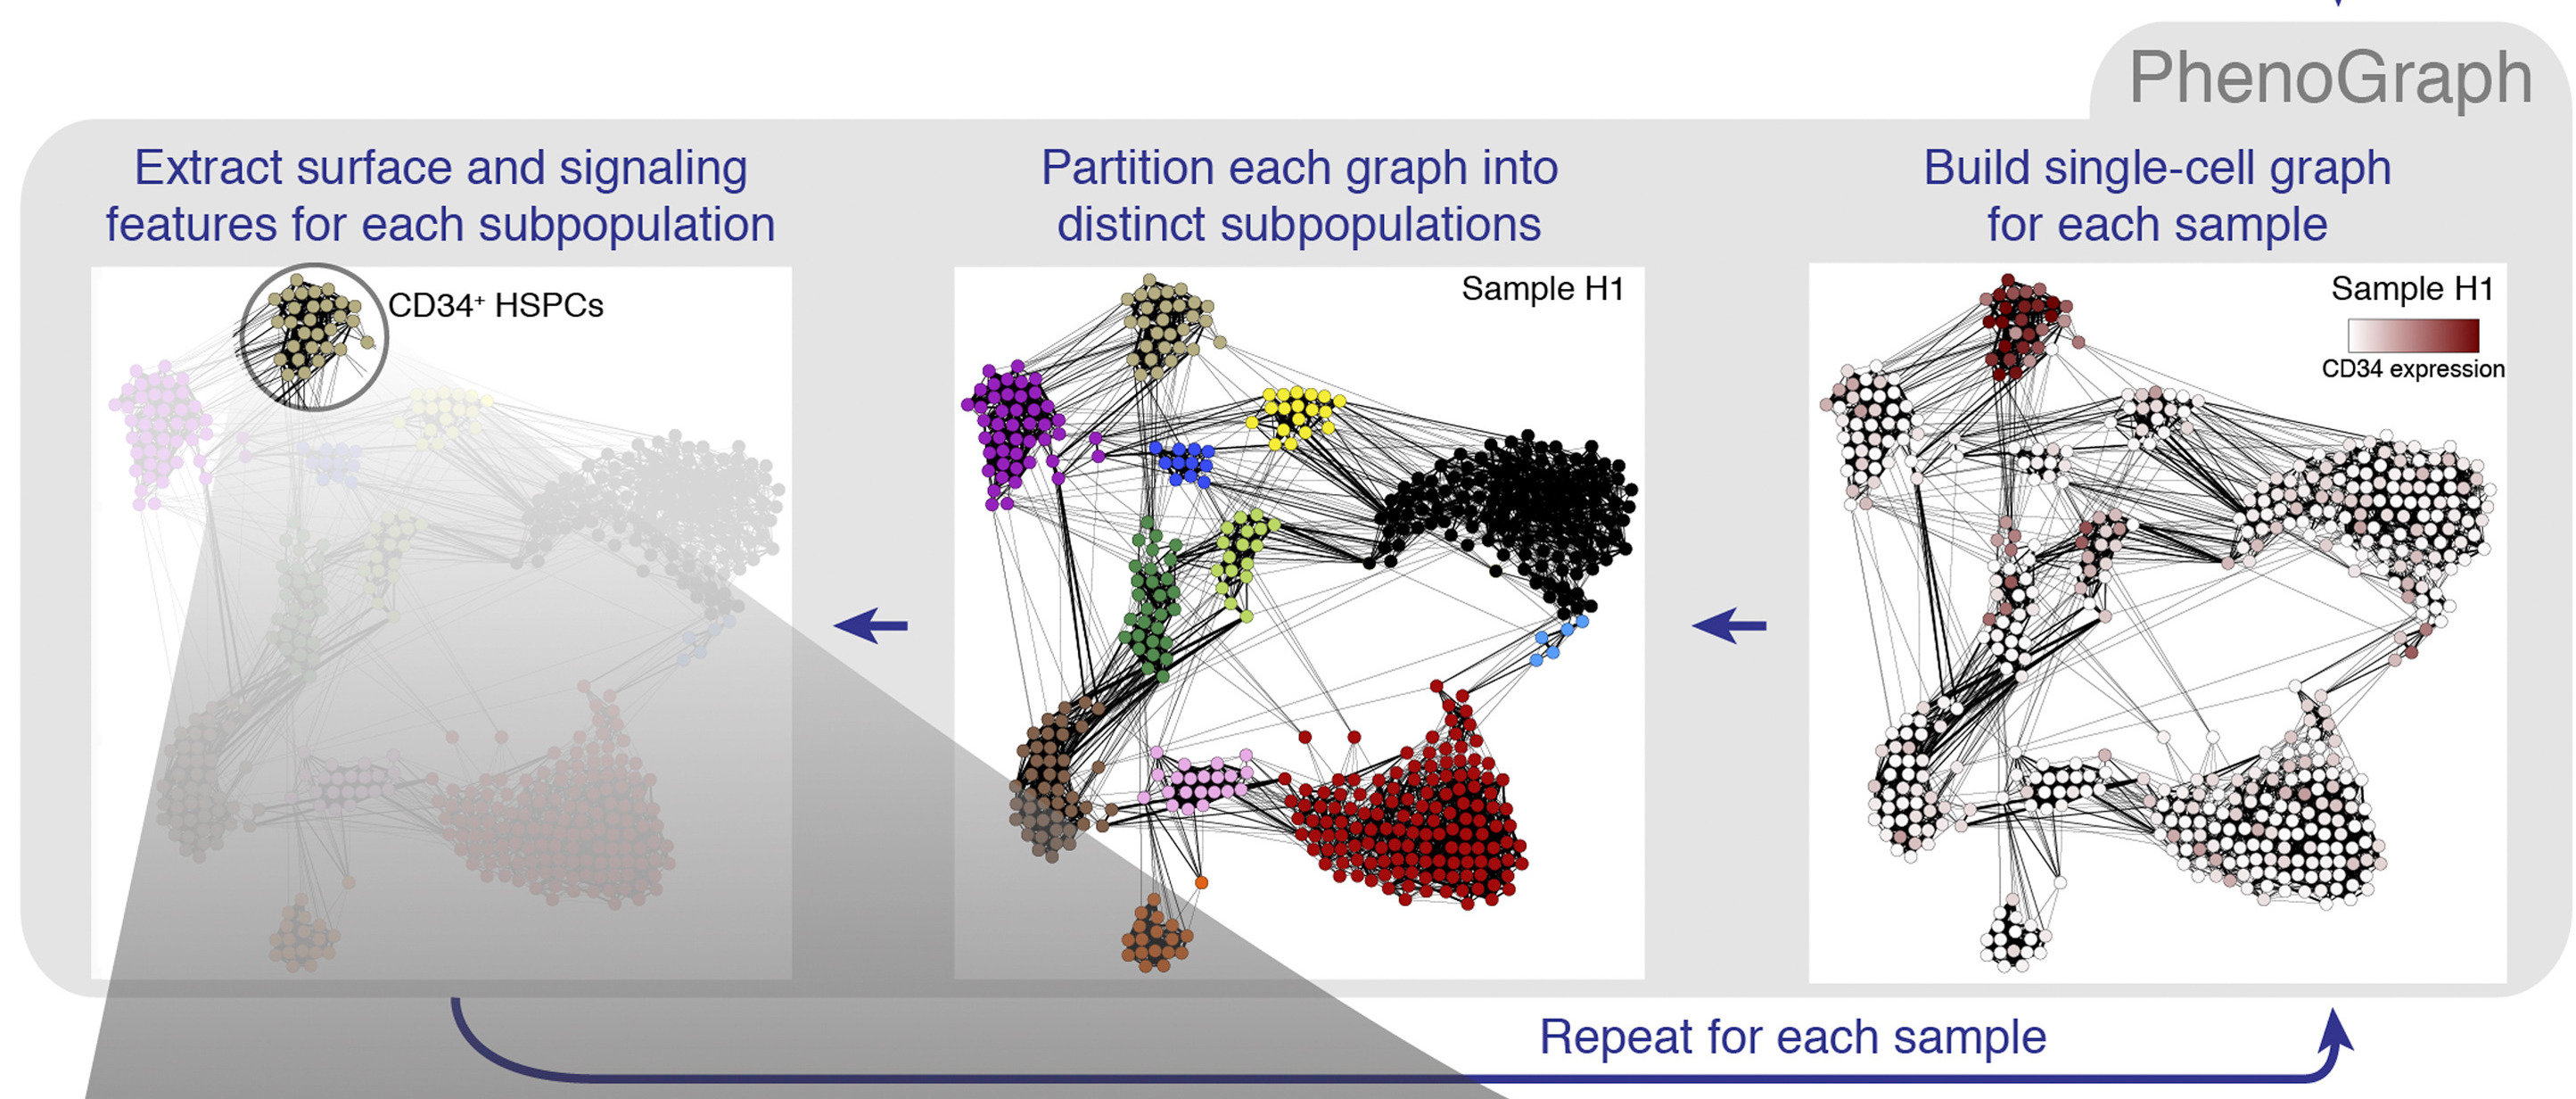
\includegraphics[scale=.72]{images/gr1_lrg_C.jpg}

\end{frame}

%--------------------------------------------------------------------------%

\subsection{1. Construcción del grafo}

\begin{frame}{Construcción del grafo: kNN}
  \vskip1em
  \begin{beamercolorbox}[sep=0.2cm,center]{coloredboxstuff}
    \textbf{Paso 1: $k$-Nearest-Neighbors}
  \end{beamercolorbox}
  \vskip-0.2cm
  \begin{itemize}
    \item $k$ vecinos más cercanos para cada célula con distancia Euclidea.
    \item Si $k$ es bajo, baja conectividad entre las poblaciones.
    \item Si $k$ es alto, resolución de poblaciones pequeñas se pierde.
    \item $N$-células con $k$-vecinos: $N$ agrupaciones.
  \end{itemize}

  \vskip0.5em
  \begin{columns}
    \hskip1.3em
    \begin{column}{0.5\textwidth}
      % \centering
      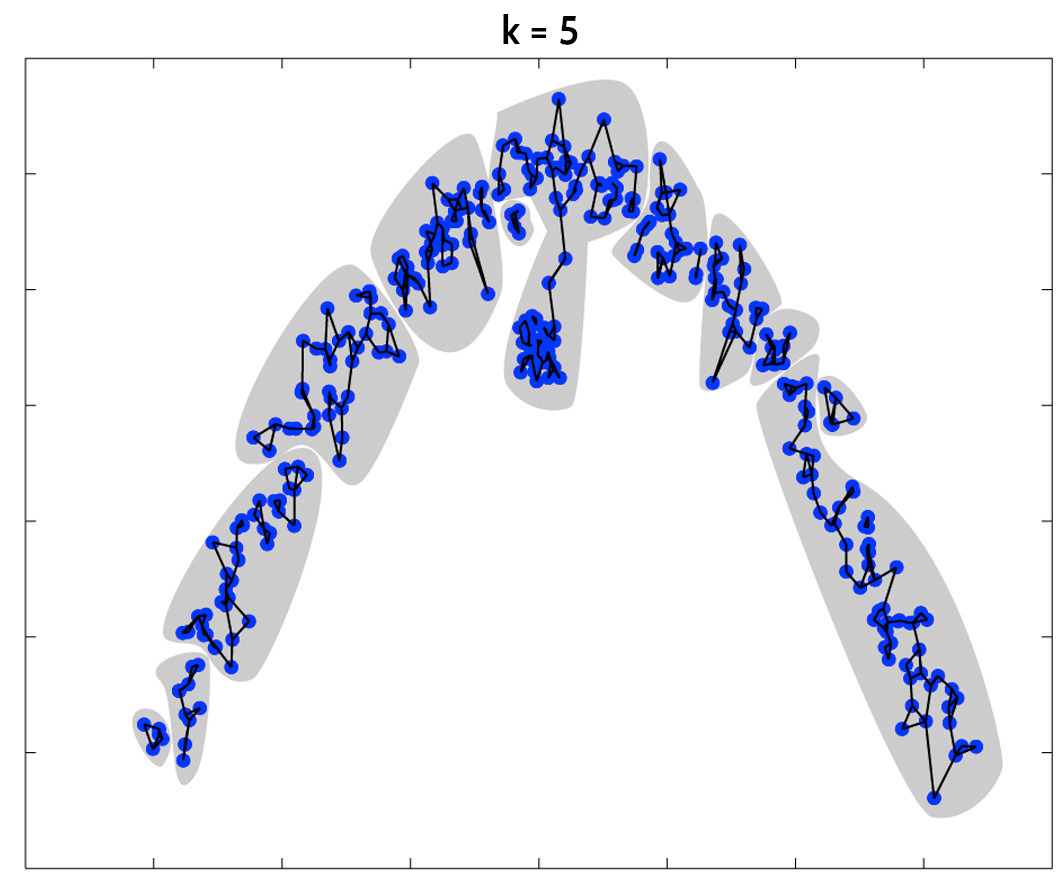
\includegraphics[scale=.9]{images/k5_knn.jpg}
    \end{column}
    \hskip-1.3em
    \begin{column}{0.5\textwidth}
      % \centering
      \vskip-0.4mm
      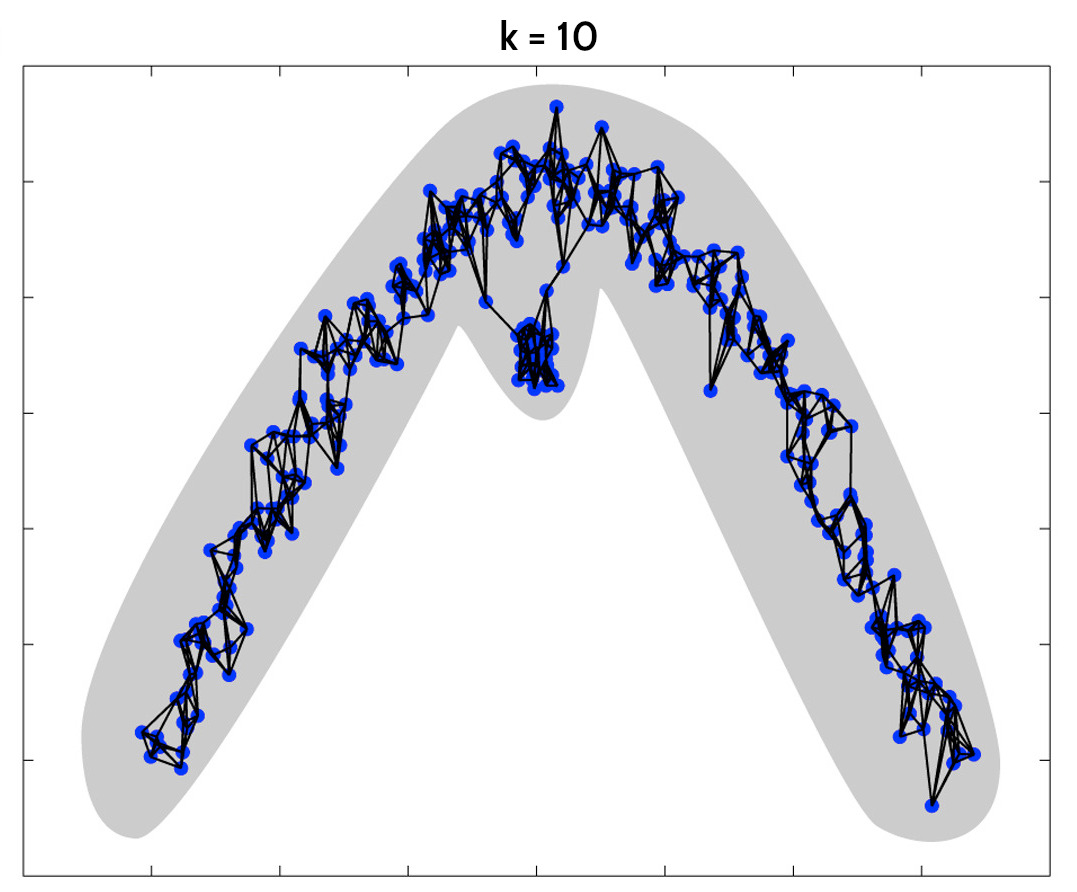
\includegraphics[scale=.9]{images/k10_knn.jpg}
    \end{column}
  \end{columns}
\end{frame}

%--------------------------------------------------------------------------%

\begin{frame}{Construcción del grafo: Coeficiente de similitud de Jaccard}
  \vskip1em
  \begin{beamercolorbox}[sep=0.2cm,center]{coloredboxstuff}
    \textbf{Paso 2: Índice de Jaccard}
  \end{beamercolorbox}
  \vskip-0.2cm
  \begin{itemize}
    \item Redefinición de $k$-vecinos de cada célula definidos por $k$NN.
    \item Índice de Jaccard: similitud entre dos conjuntos.
  \end{itemize}

  \begin{columns}
    \begin{column}{0.5\textwidth}
      \hskip8mm
      \begin{equation*}
        W_{i, j} = \frac{|v(i) \cap v(j)|}{|v(i) \cup v(j)|}
      \end{equation*}
    \end{column}
    \begin{column}{0.5\textwidth}
      \vskip0.2em
      \hbox{\hspace{-0.5em}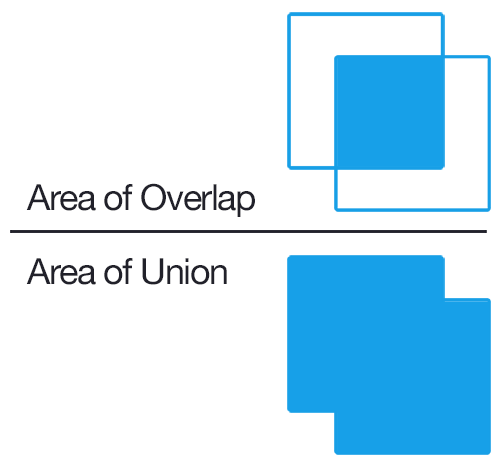
\includegraphics[scale=.2]{images/equation_jaccard_1.png}}
    \end{column}
  \end{columns}
  % \metroset{block=fill}
  \begin{textblock*}{5cm}(5.45cm,4.63cm)
    
\includegraphics[scale=0.04]{images/equal.jpg}
  \end{textblock*}
  \begin{alertblock}{Intuitivamente}
    \begin{itemize}
      \item La similitud entre células será máxima cuando sus $k$-vecinos son los
            mismos $\rightarrow$ mismo fenotipo.
      \item Similitud decaerá entre células que compartan menos vecinos conectados
            $\rightarrow$ distinto fenotipo.
    \end{itemize}
  \end{alertblock}
\end{frame}

%--------------------------------------------------------------------------%

\begin{frame}{Construcción del grafo: Coeficiente de similitud de Jaccard}
  % \metroset{block=fill}
  % \vskip-1em
  \begin{alertblock}{Resultado}
    \vskip0.20em
    Grafo ponderado con pesos basados en el número de vecinos que comparten.
  \end{alertblock}

  \begin{alertblock}{Qué conseguimos}
    \begin{itemize}
      \item Incorporamos la estructura de la distribución de los datos al grafo a
            través de los pesos.
      \item Estructura compacta y rica en información que captura la similitud entre células.
    \end{itemize}
  \end{alertblock}
  \begin{columns}
    \begin{column}{0.6\textwidth}
      \vskip-5em
      \hskip-3cm
      \begin{itemize}
        \item Se refuerzan ejes en zonas densas.
        \item Se penalizan ejes en zonas dispersas.
        \item Poblaciones raras son mejor resueltas.
        \item Outliers tienden a ser excluídos.
      \end{itemize}
    \end{column}
    \begin{column}{0.46\textwidth}
      \vskip-0.5em
      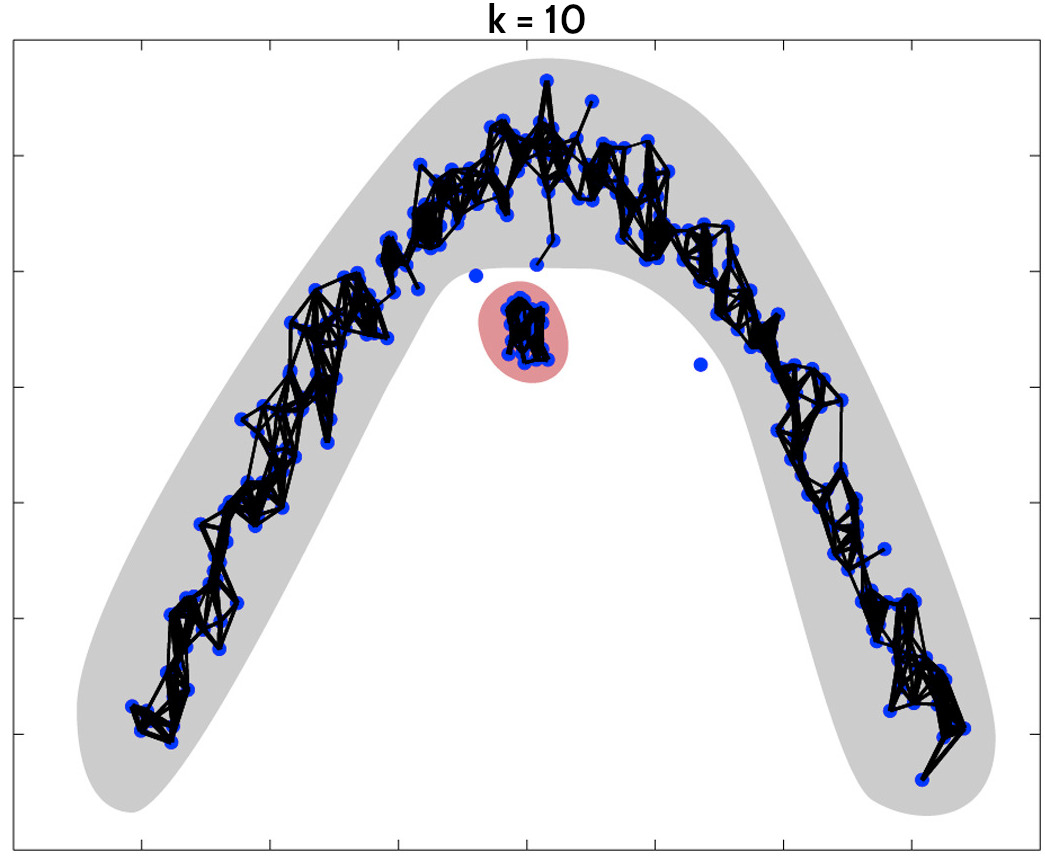
\includegraphics[scale=0.9]{images/figs1_lrg_D.jpg}
    \end{column}
  \end{columns}
\end{frame}


\begin{frame}{Partición del grafo en comunidades}
  \vskip0.2em
  \begin{alertblock}{Comunidad}
    \vskip0.5mm
    Presencia de grupos de nodos que están
    más densamente conectados entre sí que con otros nodos.
  \end{alertblock}

  \begin{columns}
    \begin{column}{0.4\textwidth}
      \vskip0.3cm
      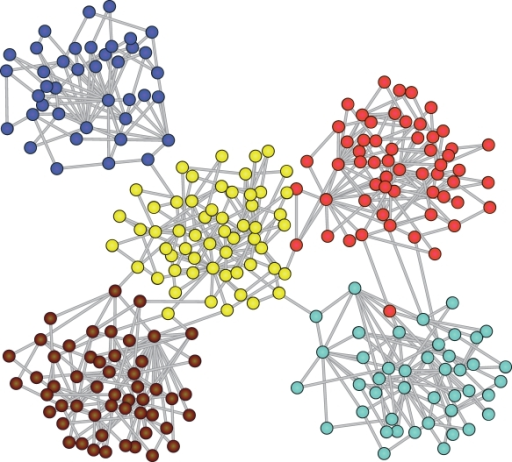
\includegraphics[scale=0.29]{images/community_graph_2.png}
    \end{column}
    \begin{column}{0.6\textwidth}
      \vspace{-3em}
      \begin{itemize}
        \item Los grafos resultantes tienen esta propiedad por cómo se han construido y
              por el tipo de datos de los que proceden.
        \item Las comunidades representan células fenotípicamente similares.
      \end{itemize}
    \end{column}
  \end{columns}
  \vskip0.5em
  \begin{beamercolorbox}[sep=0.2cm,center]{coloredboxstuff}
    Cómo encontramos las comunidades.
  \end{beamercolorbox}
  \begin{beamercolorbox}[sep=0.2cm,center]{coloredboxstuff}
    Cómo dividimos el grafo de forma óptima.
  \end{beamercolorbox}
\end{frame}


\subsection{2. Partición del grafo en comunidades}

\begin{frame}{Partición del grafo en comunidades: Modularidad}
  \begin{overlayarea}{\linewidth}{1\textheight}
    % \vskip0.2em
    \begin{alertblock}{Modularidad ($Q$)}
      \vskip0.5mm
      Medida de la calidad de una división particular de una red.
      Puede ser utilizada como función objetivo a maximizar por
      los algoritmos de detección de comunidades.
    \end{alertblock}

    % \vskip-1em
    \only<1>{
      \begin{equation*}
        Q = \frac{1}{2m} \sum_{i,j}\left[W_{i,j} - \frac{s_i s_j}{2m}\right]\delta(c_i,c_j)
      \end{equation*}
      % \vskip-1em
    }

    \only<2>{
      \vskip1em
      \centering
      \hspace{1.6em}
      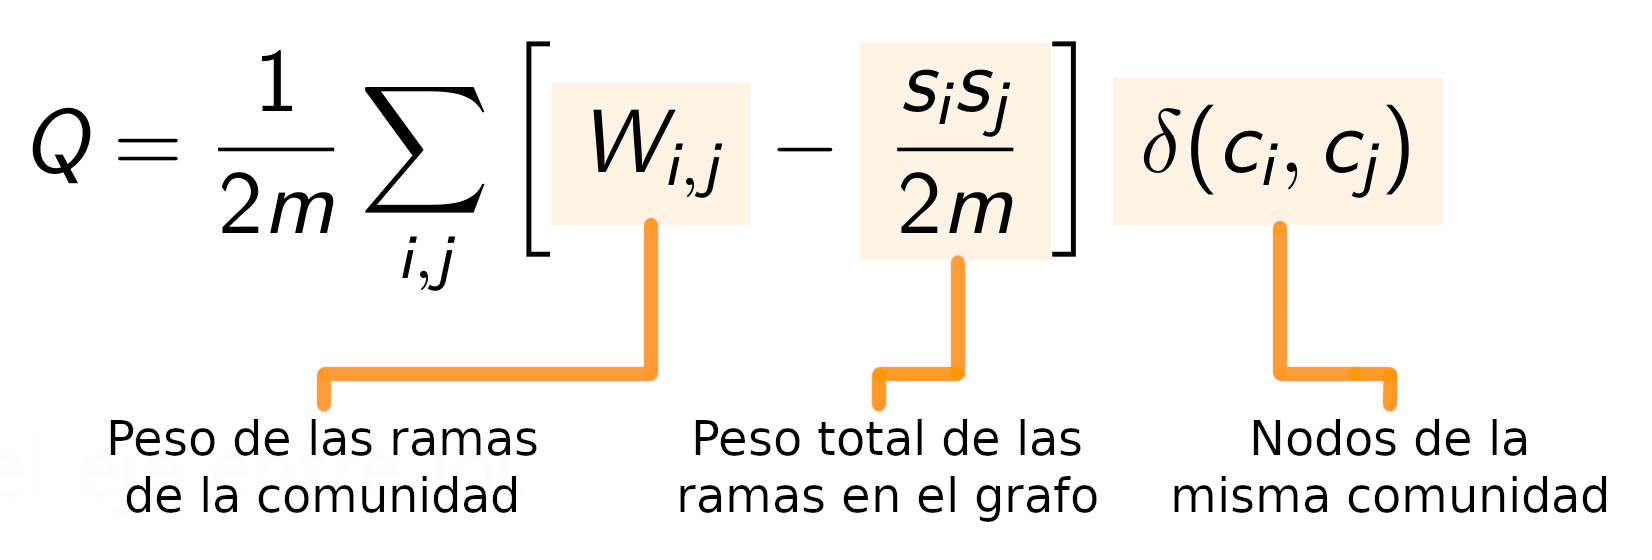
\includegraphics[scale=0.13]{images/equation_good.png}
    }
    \only<1>{
      \vskip0.5em
      \begin{itemize}
        \item $W_{i,j}$: peso del eje entre los nodos $i$ y $j$.
        \item $s_i$: suma de los pesos de los ejes que involucran al nodo $i$.
        \item $c_i$: asignación de la comunidad para el nodo $i$.
        \item $\delta(u,v)$: función delta de Kronecker: 1 si $u = v$, 0 si $u \neq v$.
        \item $m = \frac{1}{2} \sum W_{i,j}$: peso total de la red.
      \end{itemize}
    }
    \only<2>{
      \begin{alertblock}{Intuitivamente}
        \begin{itemize}
          \item Solo se calcula para pares de nodos de la misma comunidad.
          \item Cuando $W_{i,j}$ es mayor, la modularidad es más alta.
          \item Cuando $\frac{s_i s_j}{2m}$ es mayor, la modularidad baja.
        \end{itemize}
      \end{alertblock}
    }
  \end{overlayarea}
\end{frame}

\begin{frame}{Partición del grafo en comunidades: Modularidad}
  \vskip1em
  \hbox{\hspace{-0.5em}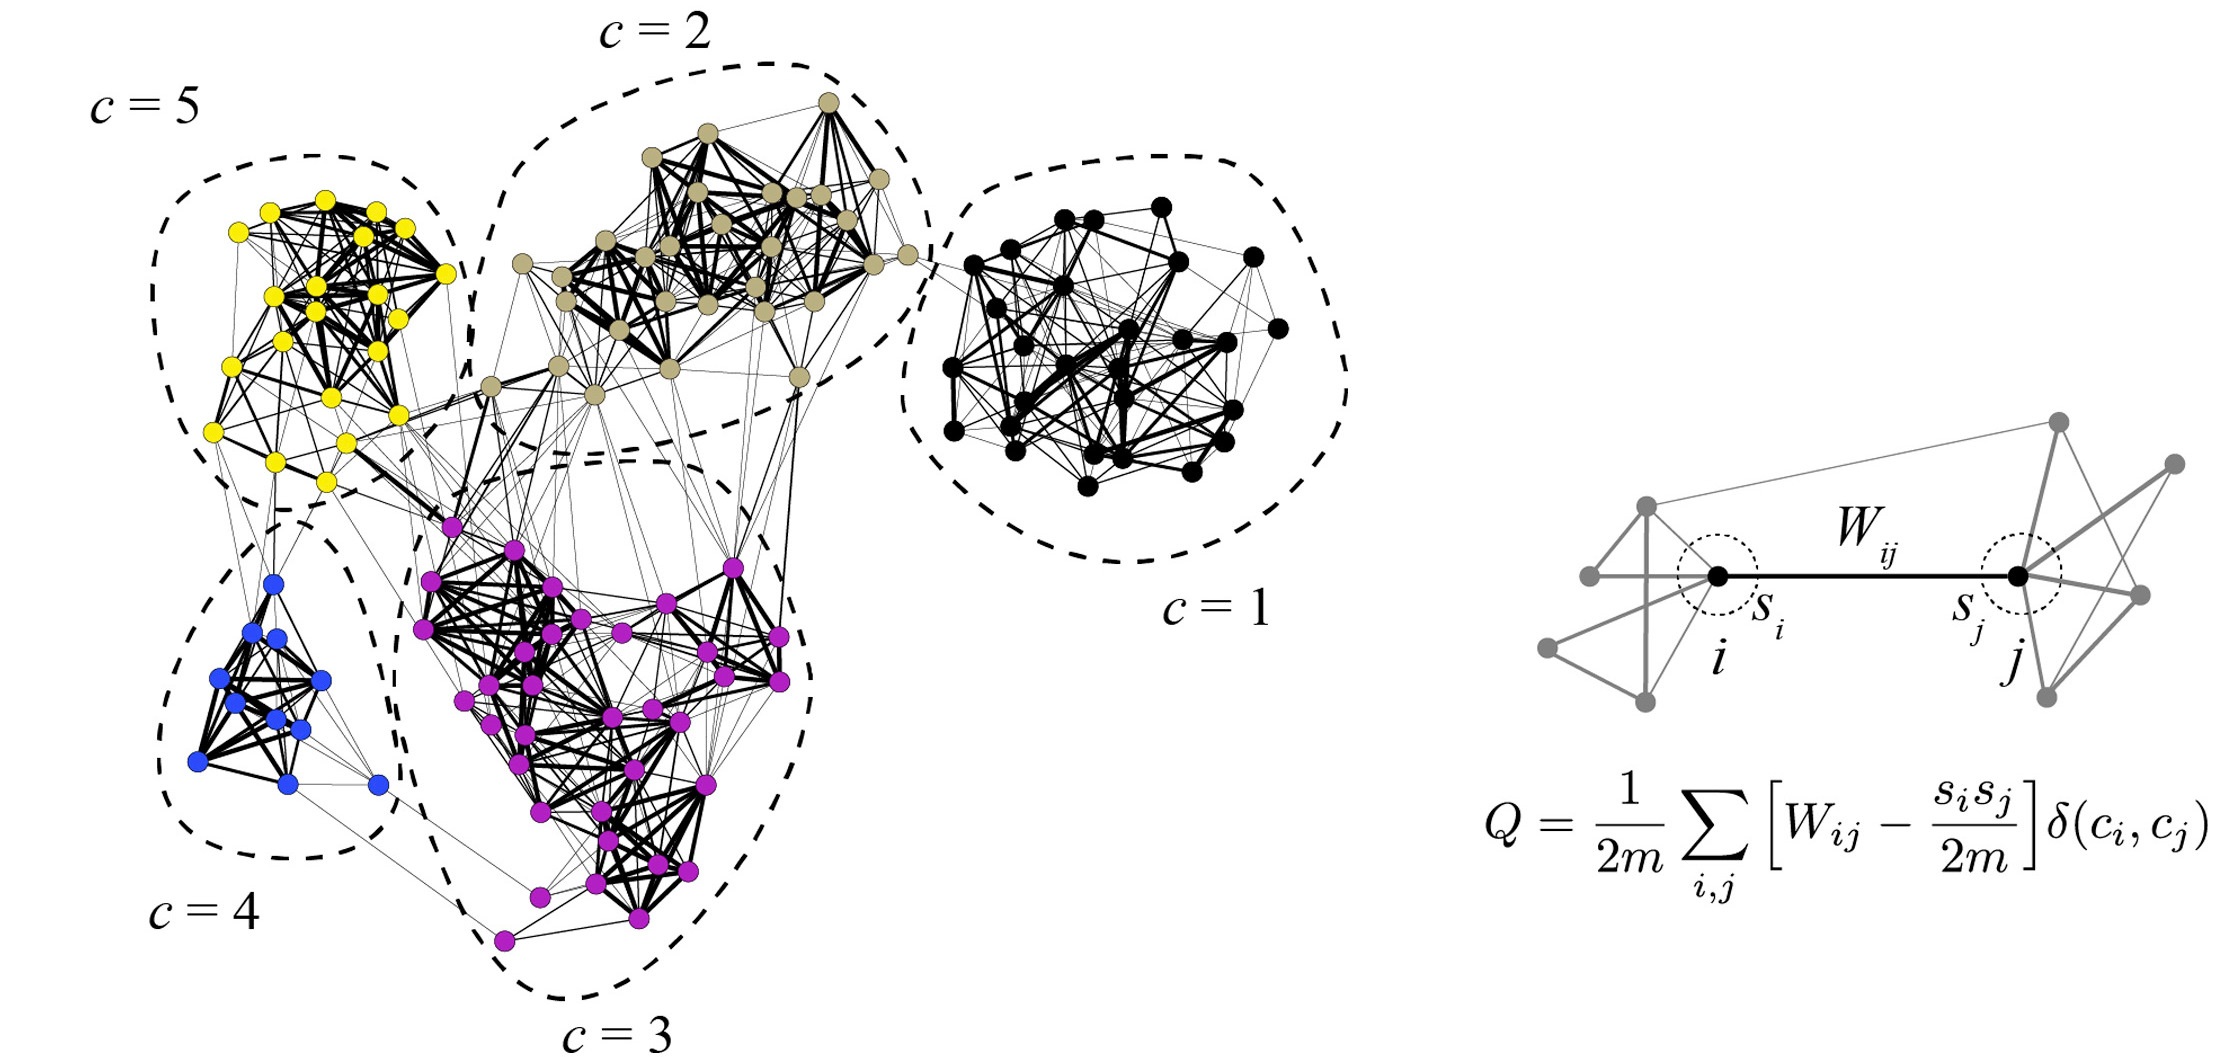
\includegraphics[scale=0.95]{images/louvain_example.jpg}}
  \vskip1em
  \begin{beamercolorbox}[sep=0.2cm,center]{coloredboxstuff}
    Búsqueda óptima: Problema de optimización combinatorial \textbf{NP-completo}.
  \end{beamercolorbox}
  \begin{beamercolorbox}[sep=0.2cm,center]{coloredboxstuff}
    Necesitamos algoritmos heurísitcos: \textbf{Método de Louvain}.
  \end{beamercolorbox}
\end{frame}


\begin{frame}{Partición del grafo en comunidades: Método de Louvain}
  % \vskip-9em
  \vskip0.2em
  Aproximación heurística con dos fases repetidas iterativamente:
  \Fonteight
  \begin{alertblock}{Primera fase}
    \begin{enumerate}[<+-| alert@+>]
      \item Se asigna una comunidad a cada nodo ($N$ comunidades).
      \item Cada nodo $i$ se asgina a la de cada vecino $j$ y
            se calcula $\Delta Q$.
      \item Si $\Delta Q$ resultante es positiva, se asigna $i$ a dicha comunidad.
    \end{enumerate}
  \end{alertblock}
  \begin{alertblock}{Segunda fase}<4->
    \vskip-0.2mm
    \begin{enumerate}[<+-| alert@+>]
      \item Se construye una nueva red con las comunidades obtenidas anteriormente
            como nodos.
      \item Los pesos se computan como la suma de los pesos de cada comunidad.

    \end{enumerate}
  \end{alertblock}
  \centering
  \vskip-1em
  % \begin{textblock*}{1cm}(3.3cm,5.8cm)
  % 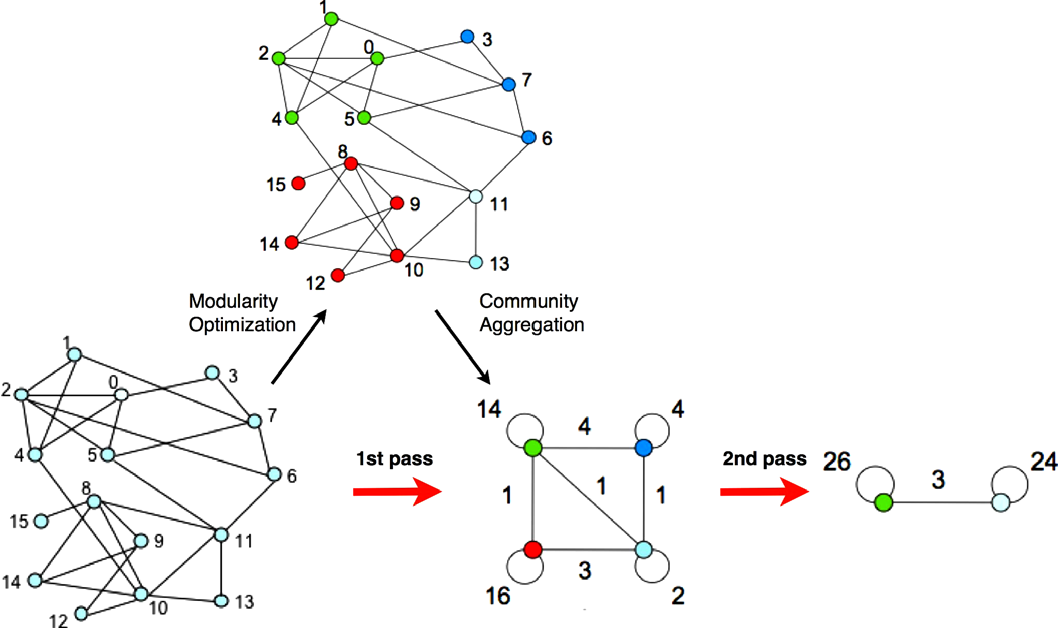
\includegraphics[scale=0.18]{images/louvine_method.png}
  \includegraphics<1,2,3>[scale=0.18]{images/louvine_method_3.png}
  \includegraphics<4,5>[scale=0.18]{images/louvine_method_4.png}
  \includegraphics<6>[scale=0.18]{images/louvine_method_5.png}
  % \end{textblock*}

\end{frame}



\begin{frame}{Pseudocódigo}
  \vskip-0.5em
  \textbf{Input:} data set of single-cell measurements $X = \{x1, .., xN\}$\\
  \textbf{Output:} subpopulation index assigning each cell in X to one of M groups\\
  \vskip2em
  \begin{beamercolorbox}[sep=0.2cm]{coloredboxstuff}
    \Fontvi
    \textbf{Inicialización:}\\
    \hspace{0.5cm}\texttt{for each cell $x_i$}\\
    \hspace{1.5cm}\texttt{find the indices ν(i) of the k nearest cells}\\
    \textbf{Construcción del grafo:}\\
    \hspace{0.5cm}\texttt{set of vertices $V = \{v_1 , ..., v_N\}$ to each cell in $X$}\\
    \hspace{0.5cm}\texttt{set of edges $E = \{\}$}\\
    \hspace{0.5cm}\texttt{for each pair of cells $x_i$ and $x_j$}\\
    \hspace{1.5cm}\texttt{compute $W_{ij}$}\\
    \hspace{1.5cm}\texttt{if $W_{ij} > 0$, add $e_{ij}$ = $W_{ij}$ to E}\\
    \hspace{0.5cm}\texttt{return $G = (V, E)$}\\
    \textbf{Detección de comunidades:}\\
    \hspace{0.5cm}\texttt{for t in \{1, ..., 100\}}\\
    \hspace{1.5cm}\texttt{decompose $G$ into $C_t$ by Louvain Method}\\
    \hspace{1.5cm}\texttt{determine best $C_t$ by maximum $Q$}\\
    \hspace{0.5cm}\texttt{return $C = C_t$}
  \end{beamercolorbox}
\end{frame}



\begin{frame}{Validación en células inmunes de adulto sano}
  \begin{overlayarea}{\linewidth}{1\textheight}
    \vskip1em
    \begin{itemize}
      \item Datos públicos: 30.000 células de médula ósea asignadas manualmente
            mediante técnicas estándar.
      \item Mayor precisión y escalabilidad que otros métodos.
      \item Robusto con diferentes parámetros.
    \end{itemize}
    \vskip1.5em
    \centering
    \includegraphics<1>[scale=0.7]{images/gr2_lrg_A.jpg}
    \vskip-1em
    \includegraphics<2>[scale=0.7]{images/histogram_performance.jpg}
    \includegraphics<3>[scale=0.8]{images/computation_time_comparison.jpg}
  \end{overlayarea}
\end{frame}



\section{Resultados}

\begin{frame}{Resultados: Datos}
  \begin{figure}
    \centering
    % \hskip-1em
    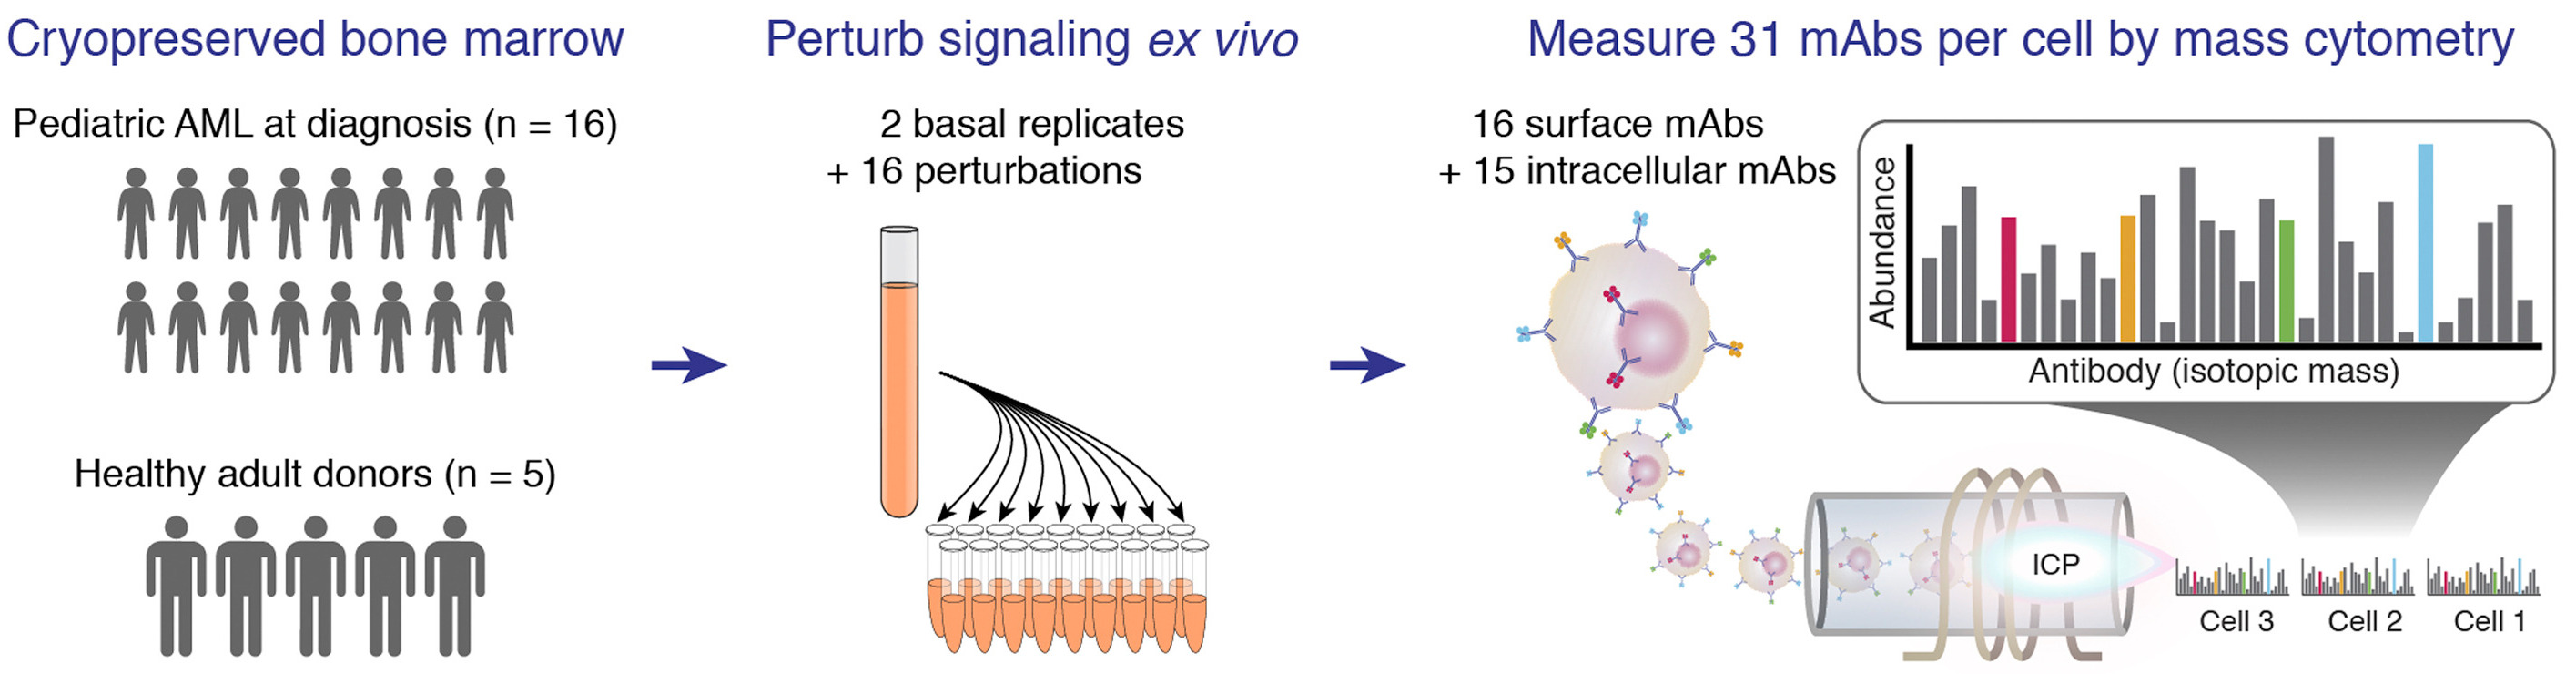
\includegraphics[scale=0.75]{images/gr1_lrg_A.jpg}
  \end{figure}
  \begin{itemize}
    \item \textbf{21 individuos:} 16 pacientes con AML, 5 adultos donantes sanos.
    \item \textbf{31 dimensiones:} \alert{16 marcadores de superficie más informativos} y 14
          sondas contra proteínas importantes en señalización intracelular.
  \end{itemize}
\end{frame}


\begin{frame}{Resultados: PhenoGraph sobre set de datos AML}
  \begin{itemize}
    \item PhenoGraph sobre la cohorte de pacientes AML y donantes sanos ($k$ = 50).
    \item 28 subpoblaciones / muestra.
  \end{itemize}
  \centering
  \vskip-0.5em
  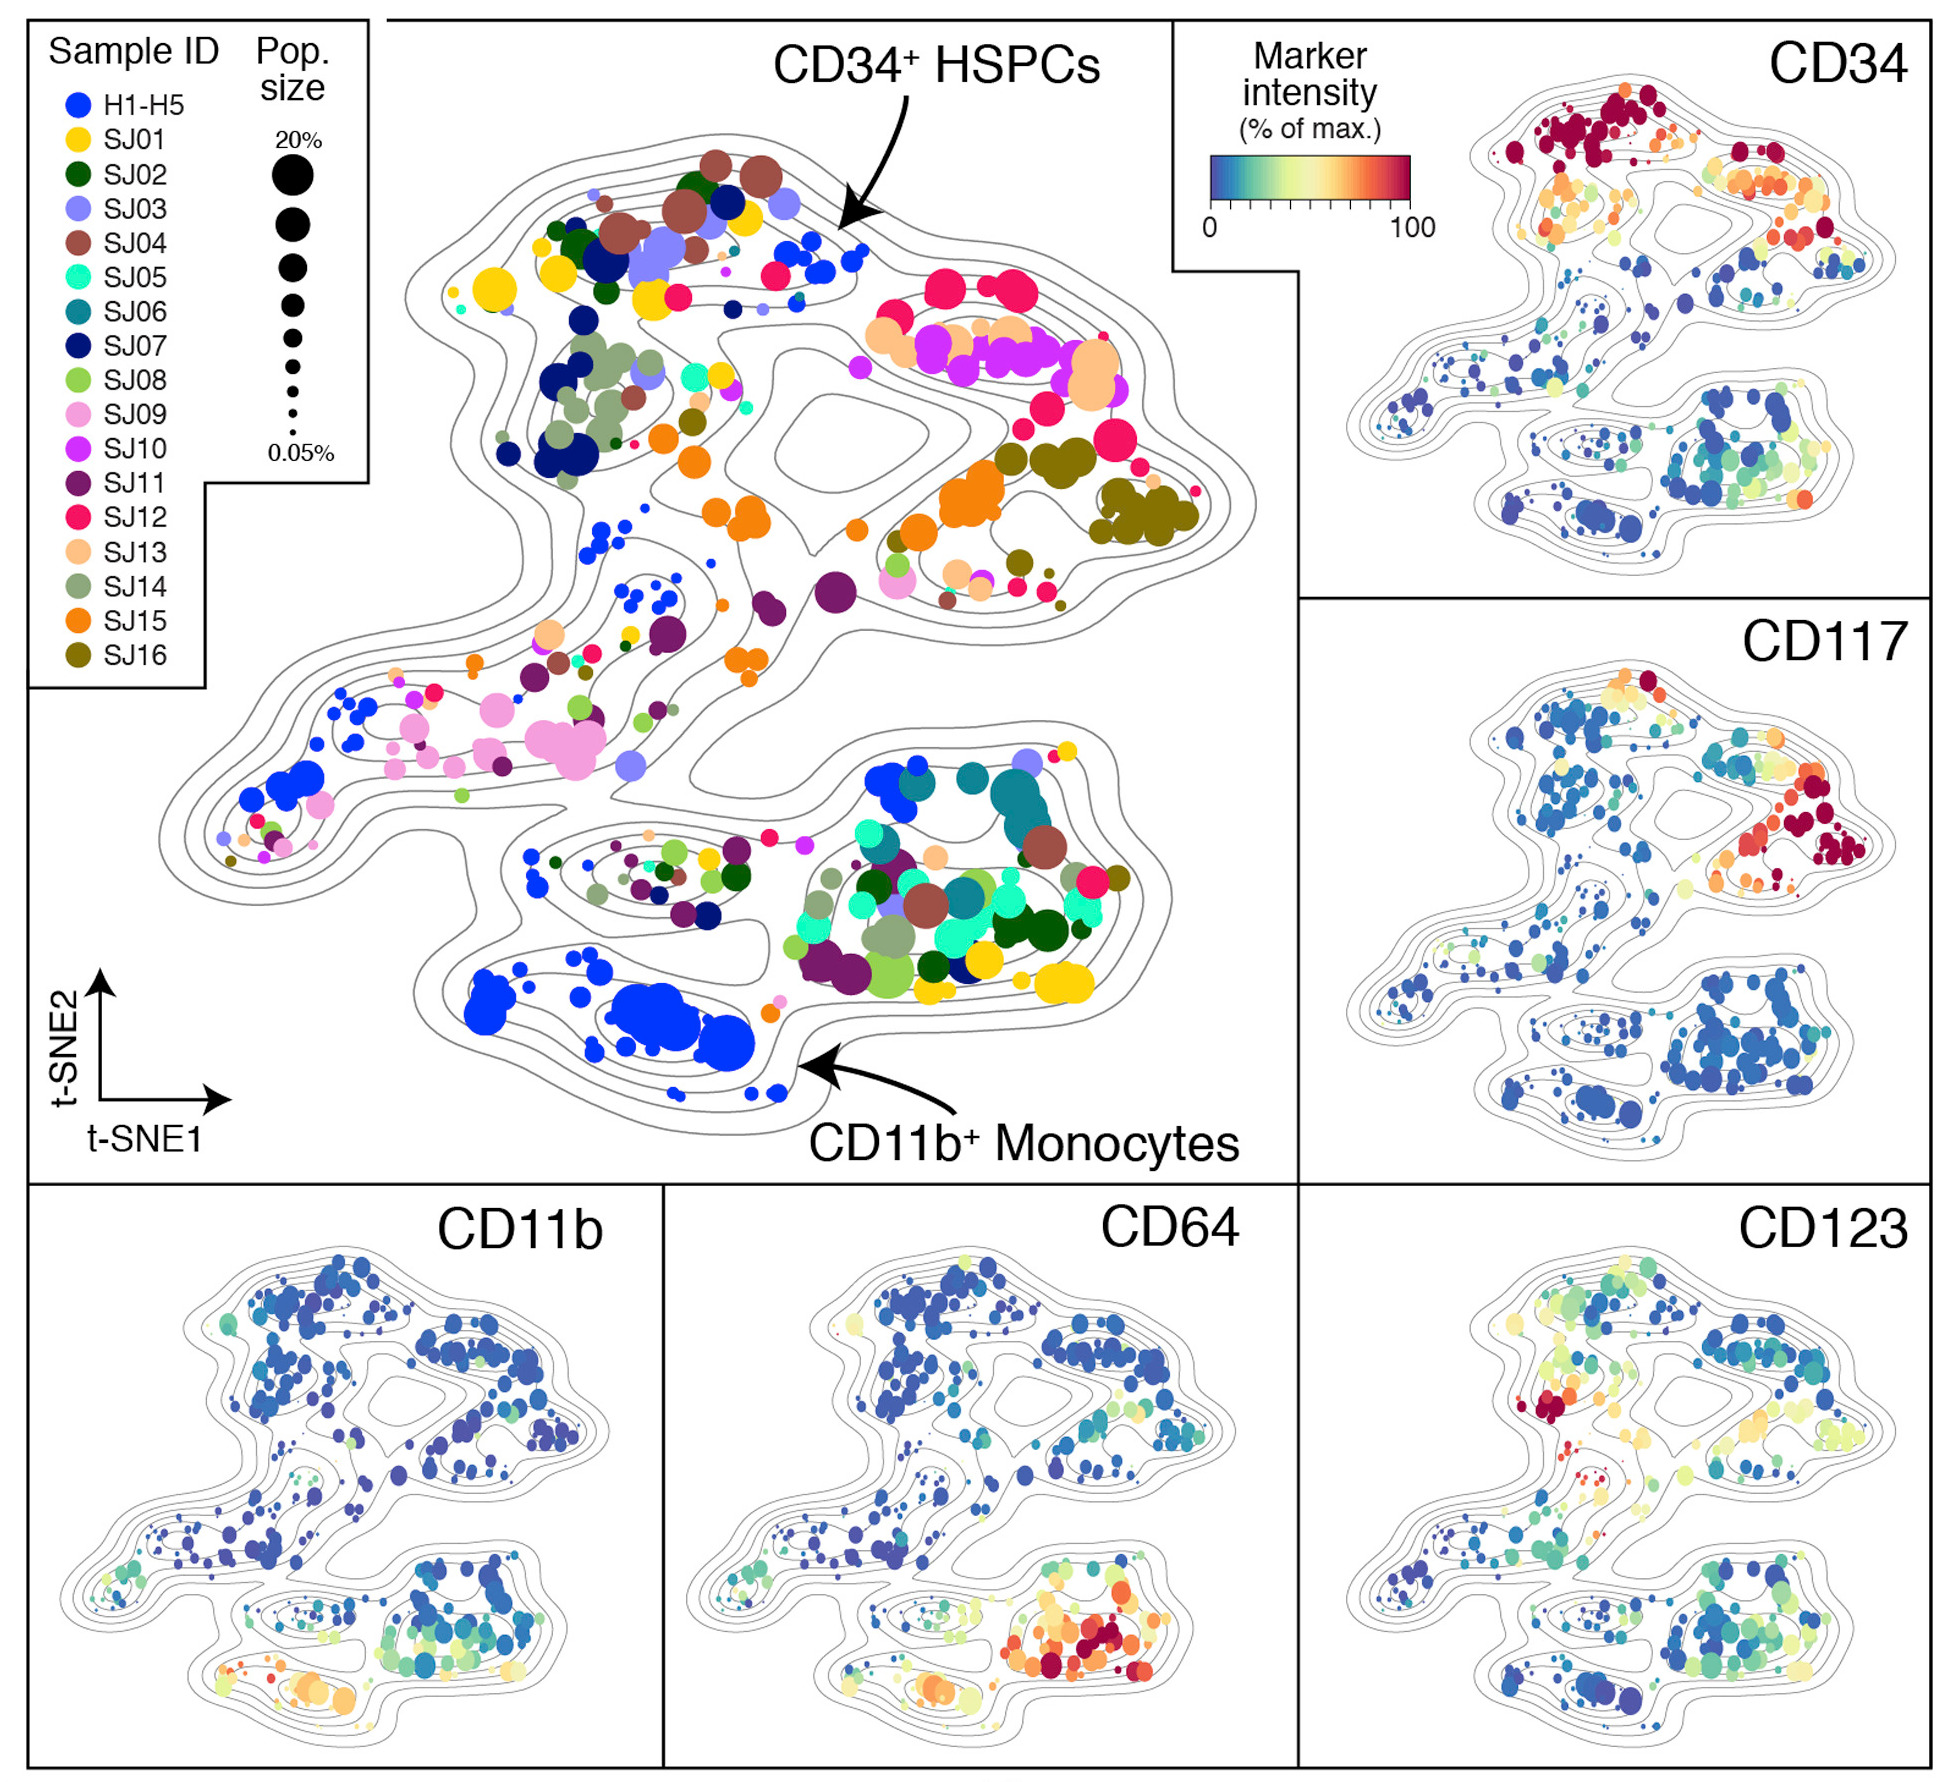
\includegraphics[scale=0.75]{images/patients_markers.jpg}
\end{frame}



\begin{frame}{Resultados: PhenoGraph sobre subpoblaciones AML}
  \begin{itemize}
    \item PhenoGraph sobre subpoblaciones AML ($k$ = 15).
    \item Cada subpoblación definida por centroides: matriz 425 x 16.
  \end{itemize}
  \centering
  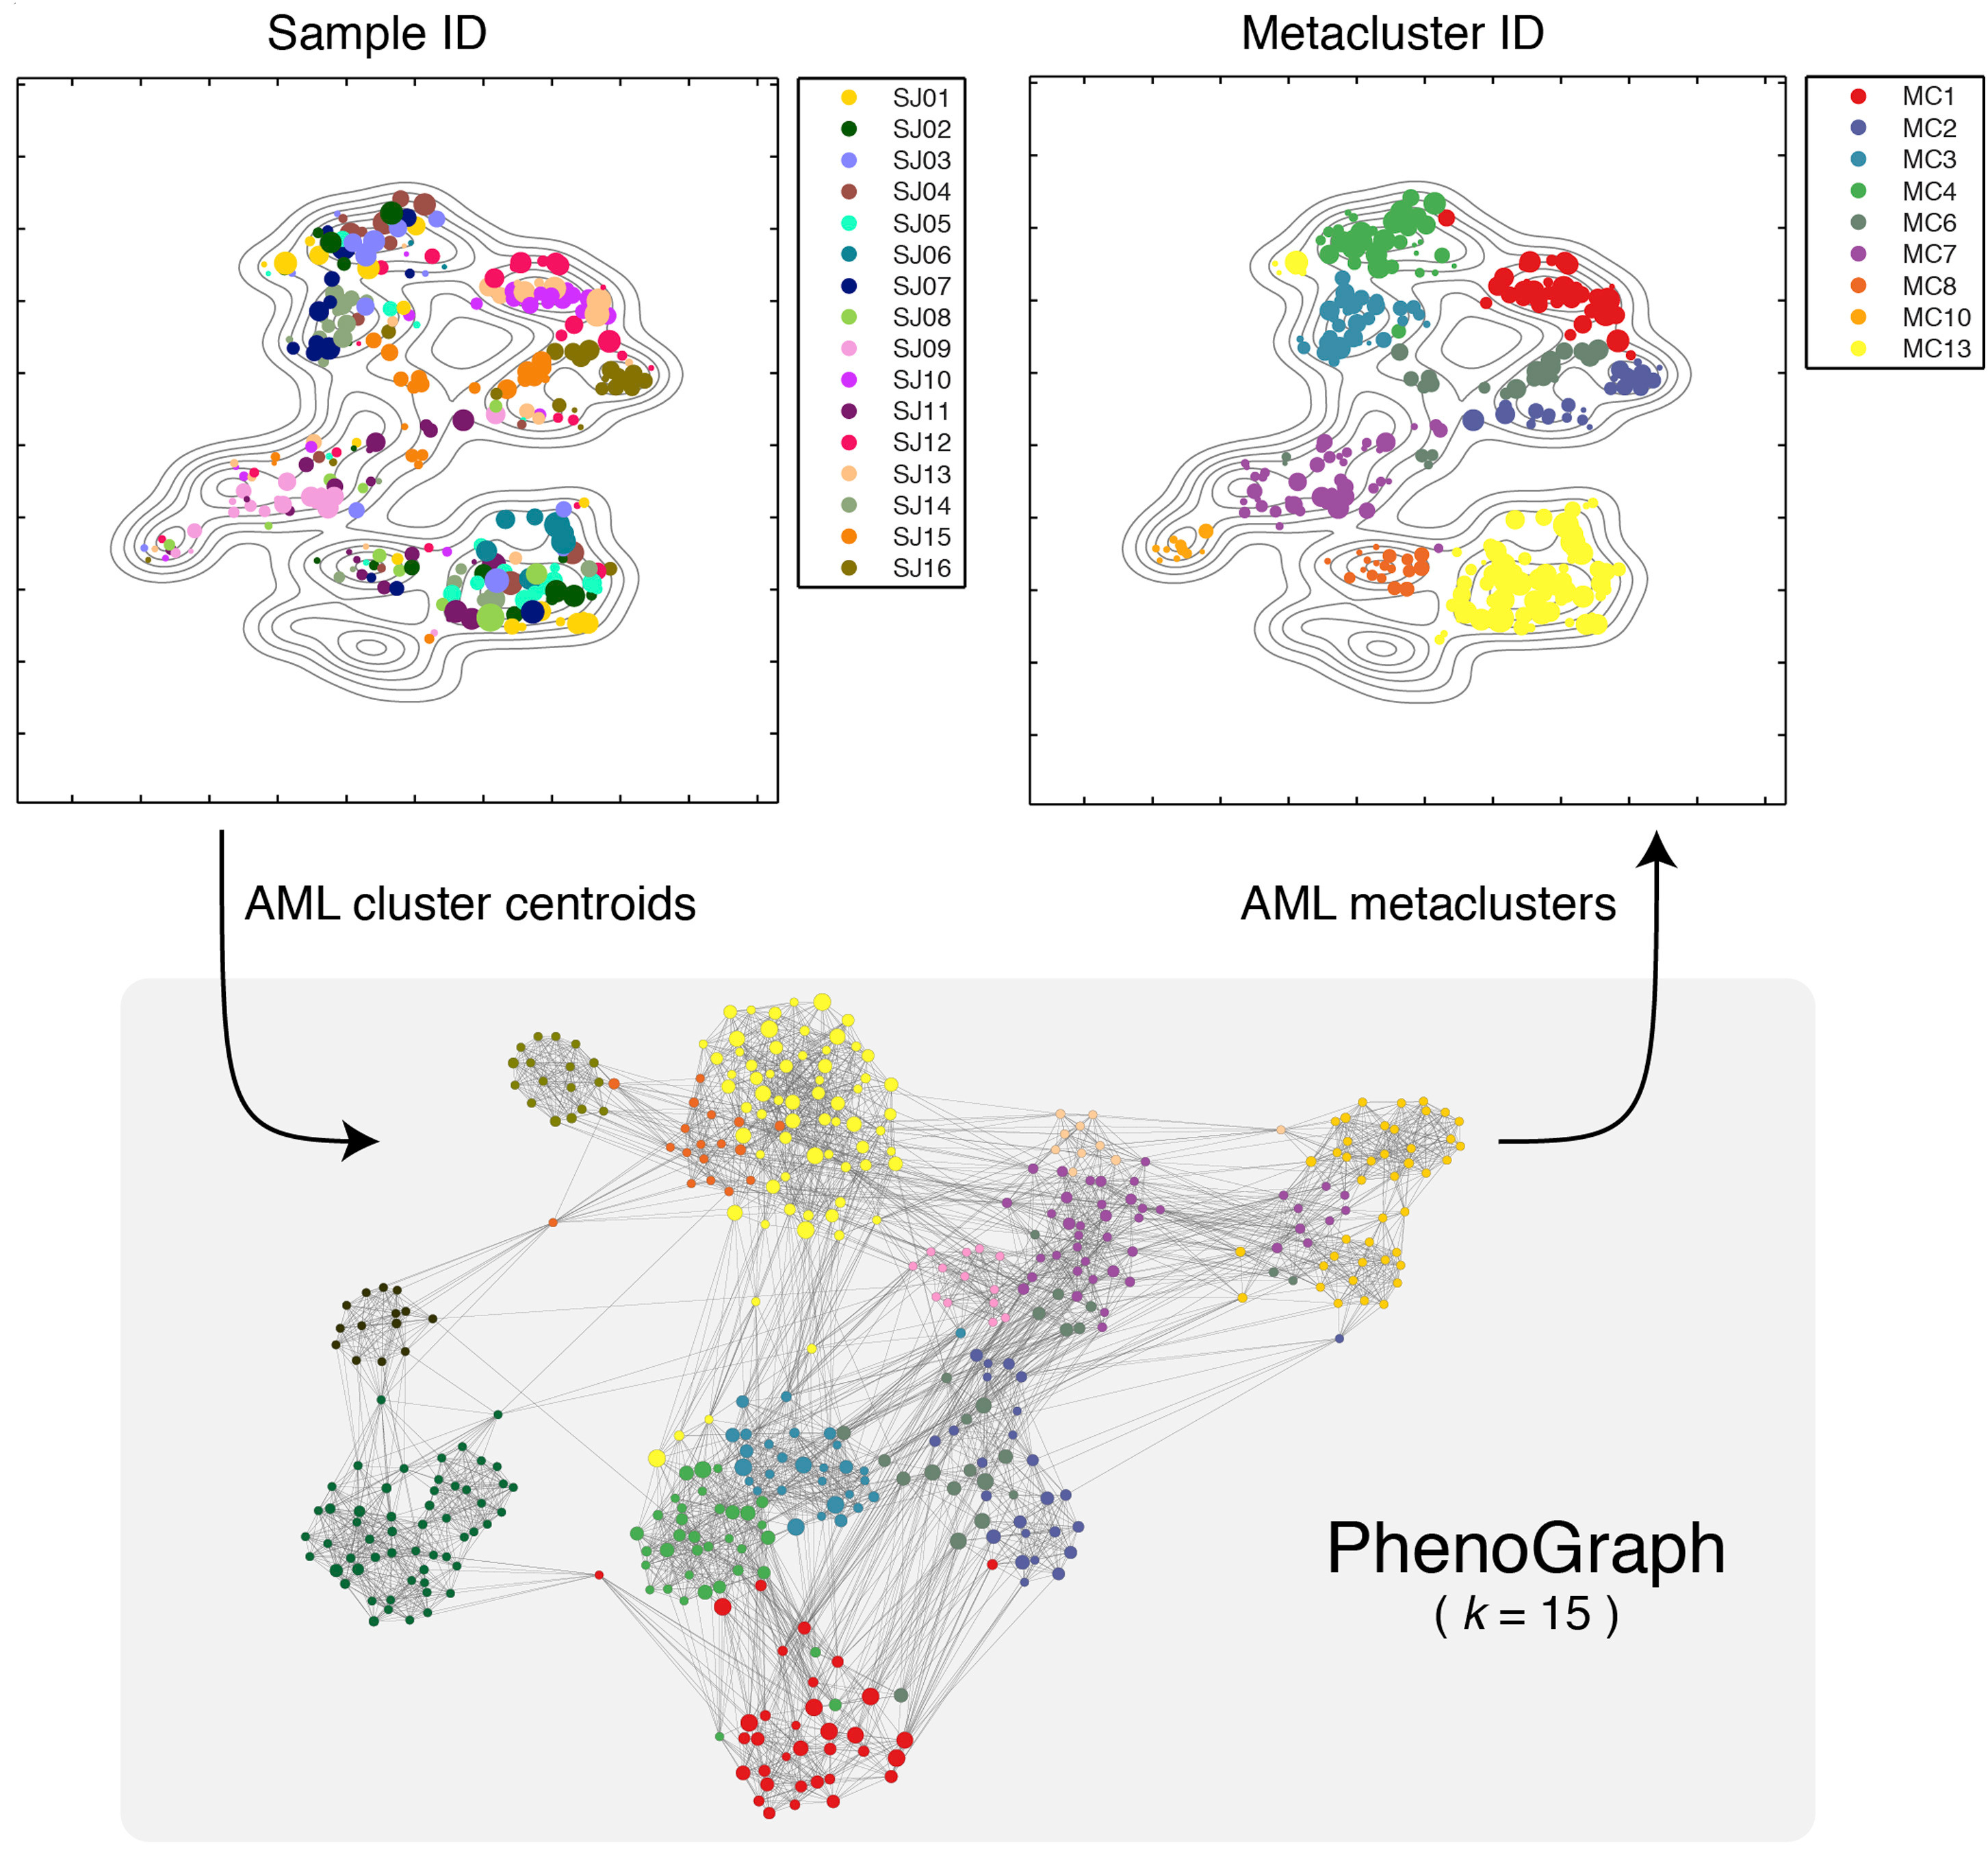
\includegraphics[scale=0.52]{images/AML_subpoblations.jpg}
\end{frame}


\begin{frame}{Resultados: Cross-validación}
  \begin{alertblock}{Resampleo de subpoblaciones AML}
    \Fontvi
    \begin{itemize}
      \item 16 repeticiones aleatorias de todos los datos.
      \item 1 paciente fuera: 16 sets de datos.
      \item 2 pacientes fuera: 120 sets de datos.
    \end{itemize}
  \end{alertblock}
  \vskip-0.5em
  \centering
  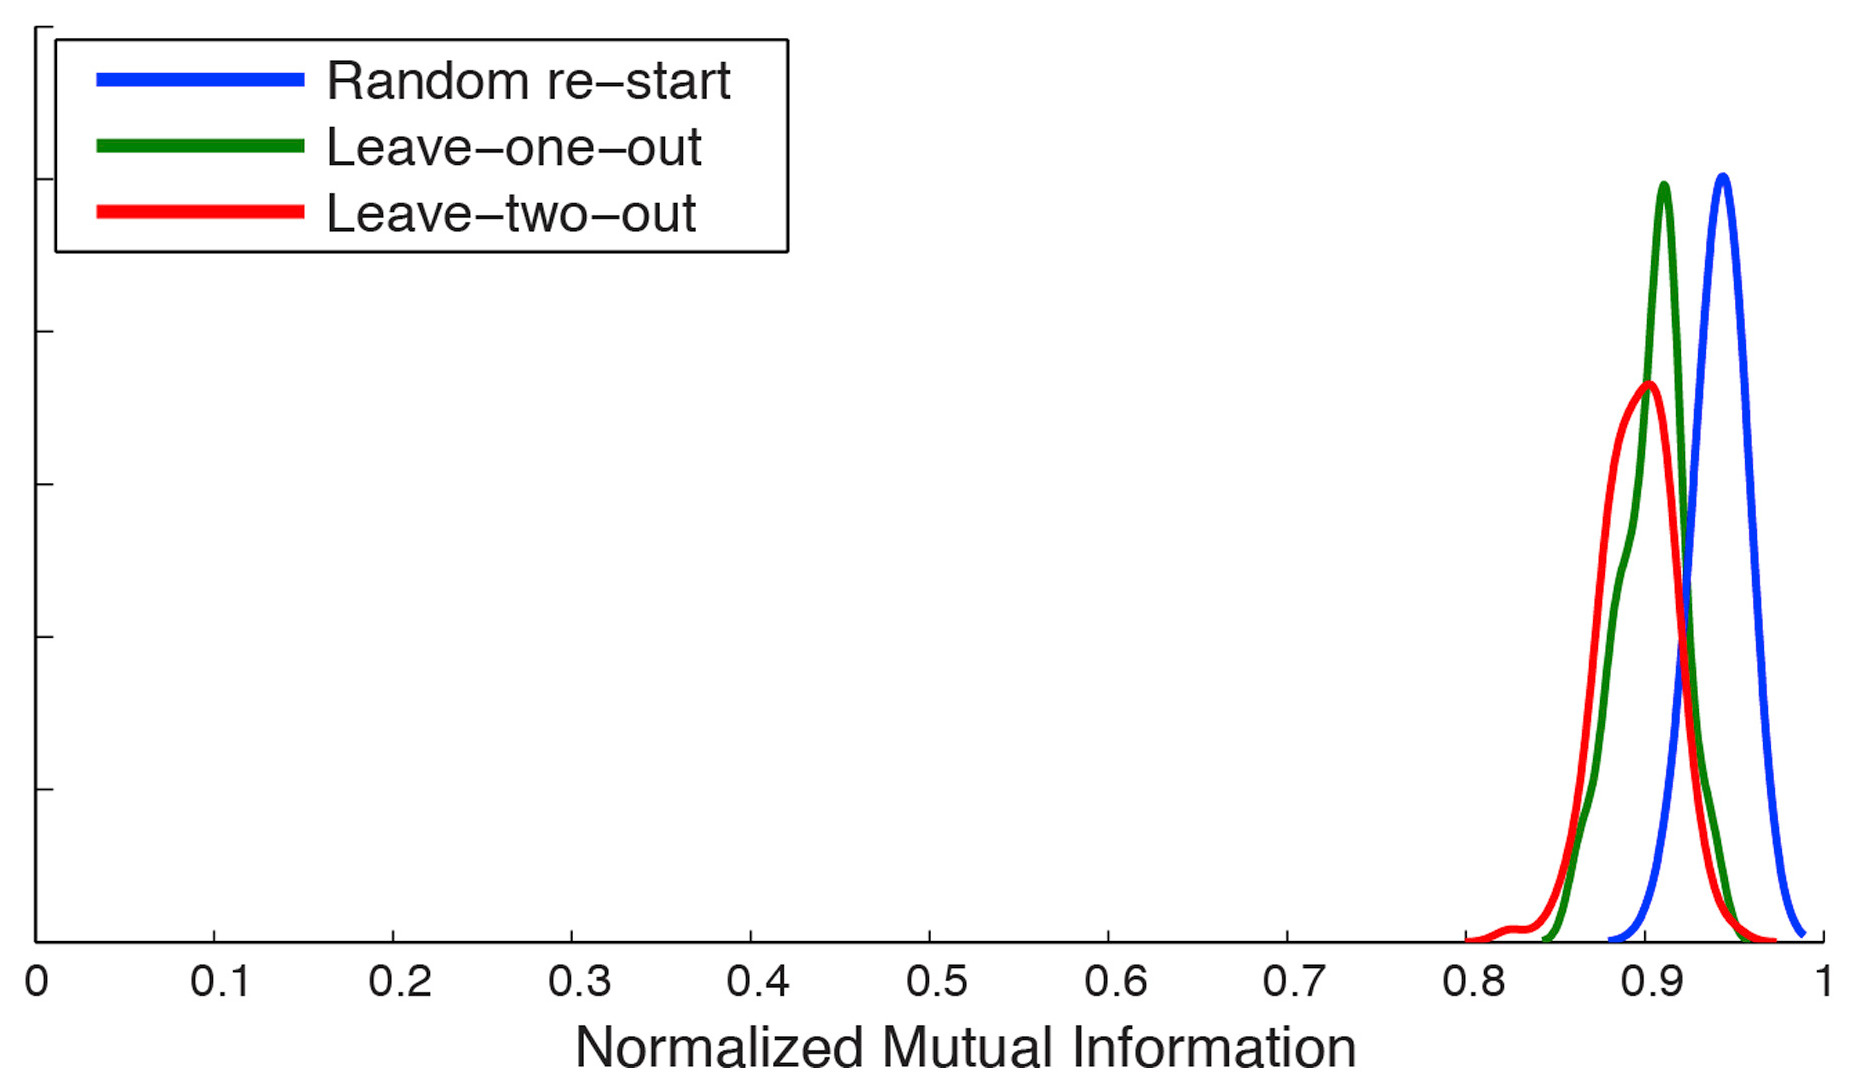
\includegraphics[scale=0.8]{images/NMI_comparison.jpg}
  \vskip0.5em
  \begin{beamercolorbox}[sep=0.2cm,center]{coloredboxstuff}
    Metaclústeres AML son robustos frente a cambios en el dataset.
  \end{beamercolorbox}
\end{frame}


\section{Otros métodos}

\begin{frame}{Comparación con otros métodos}
  % \begin{alertblock}{Papers}
  %   % \Fontvi
  %   \begin{itemize}
  %     \item A comparison framework and guideline of clustering methods
  %     for mass cytometry data.
  %     \item Comparison of clustering methods for high‐dimensional 
  %     single‐cell flow and mass cytometry data.
  %   \end{itemize}
  % \end{alertblock}

  \makebox(328,90)[rt]{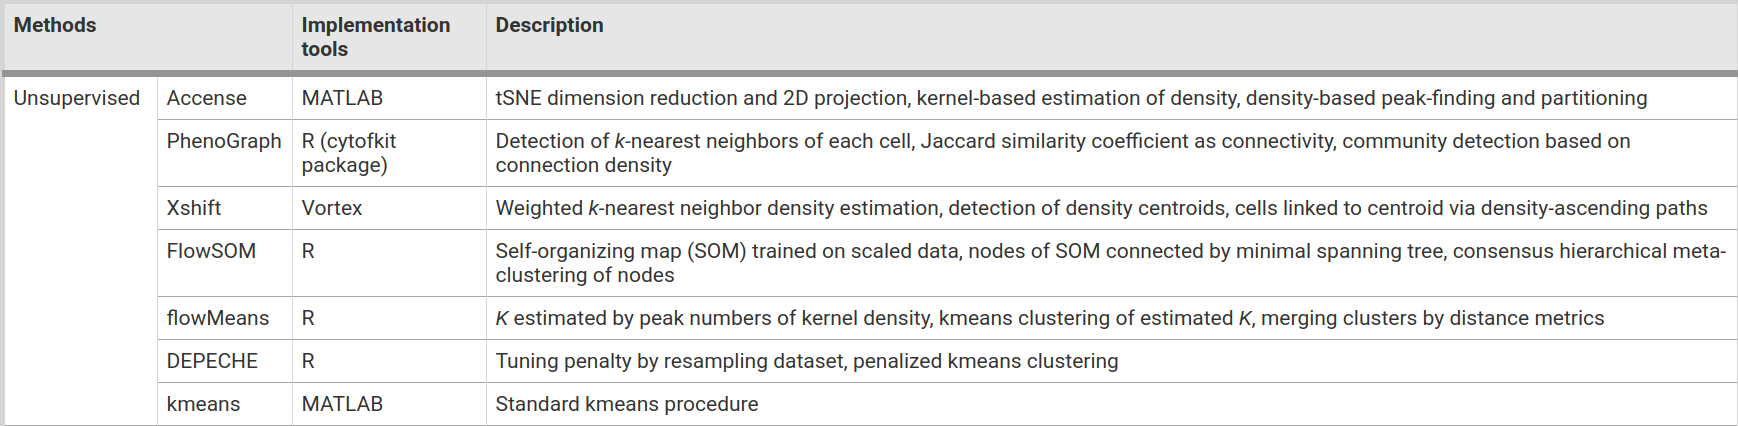
\includegraphics[scale=0.2]{images/table_methods.png}}



  \begin{alertblock}{Conclusiones}
    \begin{itemize}
      \item Robusto frente a cambio de parámetros y remuestreo.
      \item Preciso y escalable.
      \item Primeras posiciones junto a FlowSOM, flowMeans y DEPECHE.
    \end{itemize}
  \end{alertblock}
  \begin{alertblock}{Implementación}
    \vskip0.25em
    MATLAB, Python, R, paquetes de análisis scRNAseq (Seurat).
  \end{alertblock}

\end{frame}


\begin{frame}{Referencias}
  \Fonteight
  \hskip-1em
  \begin{itemize}
    \item Blondel VD, Guillaume JL, Lambiotte R and Lefebvre E. (2008). Fast unfolding of
          communities in large networks. \textit{Journal of Statistical Mechanics: Theory and Experiment}.
    \item Girvan M, Newman, MEJ. (2002). Community structure in social and biological networks.
          \textit{Proceedings of the National Academy of Sciences}. 99 (12):7821–7826.
    \item Levine JH, Simonds EF, Bendall SC, Davis KL, Amir ED, Tadmor MD, et al. (2015). Data-driven
          phenotypic dissection of AML reveals progenitor-like cells that correlate with prognosis.
          \textit{Cell}. 162:184–97.
    \item Liu X, Song W, Wong BY, et al. (2019). A comparison framework and guideline of clustering
          methods for mass cytometry data. \textit{Genome Biol}. 20:297–301.
    \item Newman, MEJ. (2006). Modularity and community structure in networks.
          \textit{Proceedings of the National Academy of Sciences}. 103 (23):8577–8582
    \item Weber LM and Robinson MD. (2016). Comparison of clustering methods for high‐dimensional
          single‐cell flow and mass cytometry data. \textit{Cytometry}. 89:1084–1096.
  \end{itemize}
\end{frame}

{\setbeamercolor{palette primary}{fg=white, bg=Blue}
\begin{frame}[standout]
  Gracias por vuestra atención.
\end{frame}
}


\appendix

\begin{frame}[fragile]{Extra}
  \begin{alertblock}{F-measure}
    \begin{align*}
      F(c_i, k_j)    & = \frac{2 \times Pr_{ij} \times Re_{ij}}{Pr_{ij} + Re_{ij}} \\
      F_{mean}(C, K) & = \sum_{ci} \frac{|c_i|}{N} max_{k_j}F(c_i, k_j)
    \end{align*}
  \end{alertblock}

  \vskip-1.5em

  \begin{alertblock}{Normalized Mutual Information}
    \begin{equation*}
      NMI = \frac{I(X;Y)}{\sqrt{H(X)H(Y)}}
    \end{equation*}
  \end{alertblock}

  \vskip-1em

  \begin{alertblock}{Non-redundancy score (NRS)}
    \begin{equation*}
      NRS(A_p) = \sum_{k = 1:c} |coeff(k)| \times eigenvalue(k)
    \end{equation*}


  \end{alertblock}
\end{frame}



\end{document}
